\chapter{\label{ch:4-methods}Methods}

%short name for attention model  -- PRALINE current favorite of the cheesy ones, but DRASC overall preferred
%Attentive recurrent splicing code
%ARSC
%Recurrent attentive splicing code
%RASC -- same as royal army service corps, favorite is this one
%For brevity, we baptise our architecture as RASC or recurrent attentive splicing code. 
%Multi-headed attentive Bi-Recurrent splicing code
%MABiRSC -- meh
%MARSC
%SCAR
%ASCR



In this chapter, we give more details about the exact task we are trying to solve, introduce the primary data sources and describe how these were used to obtain the training datasets. Additionally, we motivate and explain the evaluated models and describe how these were implemented and trained.
% We also give implementation details regarding processing steps, model implementation, and model training.

\subsubsection{Why PSI?} \label{subsubsec:whypsi}

- why not more ambitious? why not predict whole transcript directly? --> but this should be somewhere else, like in the task formulation section

ok, older works use PSI -- but why do we use it?

High-throughput sequencing methods are a popular and potent tool to investigate RNA expression and post-transcriptional regulation. However, due to limited coverage, short read length, and experimental biases they are not able to provide a full view of post-transcriptional processing so far \cite{berlinpsi}.
-> this is why you introduce alternative splicing events; as reads are too short to identify splicing events


\section{Task formulation} \label{sec:task_formulation}
The output of our models will be the classification of a given exon or junction as constitutive or non-constitutive. To obtain the training label of an exon or junction as constitutive or non-constitutive, we need its respective PSI value. 
Strictly speaking, all exons and junctions with a PSI of less than 100\% are non-constitutive. However, due to spurious reads, we classify all exons with a PSI $\leq 99\%$ as constitutive. 

Previous work indicates that advances in predicting one type of alternative splicing behaviour (e.g. cassette exons) via Machine Learning methods also translates to advances in prediction for other types (e.g. exons with an alternative 3' splice site) \cite{dsc} \cite{buschhertel}. Therefore, a practical choice is to only focus on one splicing type as this reduces the number of experiments and needed training time by two to three factors. As noted, cassette exons are the most common form of alternative splicing in higher eukaryote and thus we choose cassette exons as the type of alternative splicing we will focus on.

\section{Datasets}\label{sec:datasets}
Three primary sources for genomic data were used in this study: the Human Exon splicing events (HEXEvent) database \cite{hexevent}, data from the Genotype-Tissue Expression (GTEx) project \cite{gtex} and data from the Human Induced Pluripotent Stem Cell Initiative (HipSci) \cite{hipsci}. Except for the HEXEvent database, none of these primary sources directly report the PSI values of exons or junctions. However, we will use the PSI value as our prediction target and thus apply further processing steps to obtain PSI estimates \ref{subsec:psiestimation}. All of the data sources required further processing (e.g. extraction of corresponding nucleotide sequences) to obtain the final samples which are the input for the models. These further processing steps are described in section \ref{subsec:finalsampleprocessing}.


\subsection{HEXEvent database} \label{subsec:hexevent}
The HEXEvent database contains genome-wide exon data sets of human internal exons which can be filtered for selected splicing events (e.g. constitutive or cassette exons). It was compiled based on known mRNA variants as defined by the UCSC Genome Browser (newest version is hg38) as well as their associated available expressed sequence tag (EST) information. ESTs are short cDNA sequences which have been used in older sequencing techniques (before the advent of modern high-throughput sequencing technologies). 

%TODO perhaps extra section where I discuss the merit of each dataset because right now it doesn't fit
Some issues with ESTs which therefore also affect HEXEvent are worth highlighting. EST are based on only a single sequencing pass and especially bases at the 3' and 5' end of the EST are known to be highly error prone \cite{hitchhiker}. Additionally, ESTs underpresent less frequent transcripts and as a result often only capture 50 - 65\% of an organism's genes \cite{estunderrepresenttransripts}. Thus, these biases may also have an adverse effect on the HEXEvent database's data quality.

%Thus, great care needs taken to account for these systematic biases when working with EST data.
%It was chosen as a data source for direct comparability with the baseline paper \cite{dsc}.

%EST underrepresent rare transcripts and often only account for 60\% of an organism's genes, yep 50-65\%
%- EST seqeuence;very short and highly error prone especially at the ends
%EST also permits low quality bases due to single pass sequencing, and some sequences are highly redundant in certain genes.
%- what sort of processing against bias does hexevent do?


%these are sequence reads datasets based on which I will estimate the PSI values
\subsection{GTEx} \label{subsec:gtex}
The GTEx project provides the most comprehensive database for tissue-specific gene expression and regulation available to-date; containing over 17000 samples from nearly 1000 human donors. The sequencing data was obtained using mainly molecular assay-based techniques like Whole Genome Genotyping (WGS), Whole Exome Sequencing (WES) and RNA-Seq. Samples were taken from up to 54 different tissue sites. In particular, the tissue samples are also taken from less commonly seen tissue sites such as brain or heart as the GTEx project sources its samples from recently-deceased donors who have donated their body to science. Thus, the GTEx project, and by extension the parts of this thesis relying on GTEx data, was only made possible through the kindness and generosity of donors making their body available for science.

Processed data which can not be used to identify the donors is publicly available on the GTEx portal. To access raw data (e.g. raw RNA-seq reads) and meta-information about the samples one is required to undergo a data access request. It is intended that data access is requested by PIs or leader of research groups for their whole lab and approval of a data access request usually takes upwards of 3 months. The co-collaborators Prof. Wilfred Haerty and Prof. Elizabeth Tunbridge have access to the protected part of the GTEx data. However, the scope of projects for which they were granted access does not include this thesis and changing the scope would require undergoing the data access process again. For this reason, we can only use the publicly available part of the GTEx data in this study, in particular the files containing information about exon-exon junction reads. 

%using gtex:
%'We strongly recommend the use of TPM (Transcripts Per Million), because is normalized for gene length first, and then for sequencing depth. This allows a direct comparison between samples' https://github.com/comprna/SUPPA/wiki/SUPPA2-tutorial
%good site: https://www.ncbi.nlm.nih.gov/projects/gap/cgi-bin/study.cgi?study_id=phs000424.v8.p2
\subsection{HipSci} \label{subsec:hipsci}
%TODO is my interpretation that iPSC cells are differentiated to neurons actually correct? -> perhaps ask in meeting
% https://www.biorxiv.org/content/10.1101/095943v1 iPSC-derived sensory neurons; http://www.hipsci.org/lines/#/lines/HPSI0114i-eipl_1
\begin{figure}
	\centering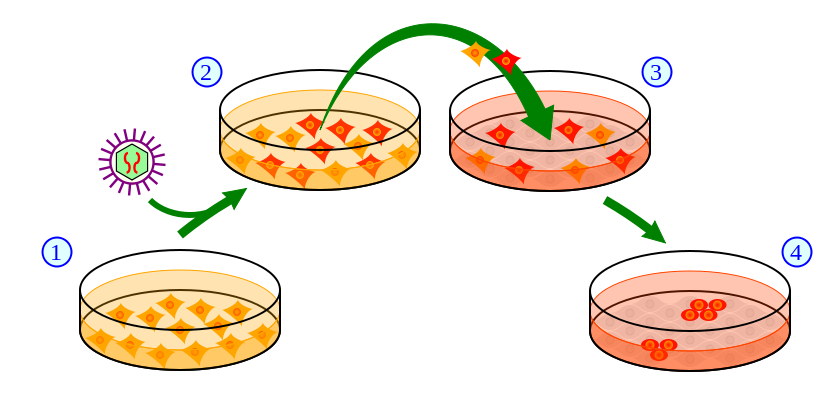
\includegraphics[width=0.7\textwidth]{../visualizations/ch4-methods/ipscprocess.png} 
	\caption[test.]{
	The four high-level steps taken to obtain iPSC cells \cite{img:ipscprocess}:
	(1) Grow a cell culture of donor cells, (2) transduce the genes associated with reprogramming into the cells via viral vectors, (3) isolate the cells expressing the transduced genes (in red) and culture them according to embryonic stem cell culture and, finally, (4) a small subset of the transfected cells become iPSC cells.
}
	\label{fig:ipscprocess}
\end{figure}

HipSci provides a large repository of human induced pluripotent stem cell (iPSC) lines. iPSC cells are mature cells which have been reprogrammed to again become pluripotent (undetermined). This process is visualized in Figure \ref{fig:ipscprocess}. As iPSC cell lines are not directly obtained from human donors, but rather from building a cell culture based on some initial donor cells, accessing raw RNA-seq reads is not constrained by the same data privary regulations which prevented access to the raw RNA-seq reads from the GTEx project.


Concretely, over 300 cell lines from over 300 donors along with sequencing information based on RNA-seq is publicly available from the HipSci portal. From these we selected two different groups of cell lines:
\begin{itemize}

	\item the first group contains 25 biological replicates (that is, samples from different cell lines developed under the same conditions) of sensory neuron cell lines \cite{ipscneurons}. These cell lines were obtained by differentiating iPSC cells to sensory neuron cells.
	\item the second group contains 20 biological replicates of iPSC cell lines which weren't differentiated to any other cell type. Here care was taken to choose donors from whom at least two different iPSC cell lines were developed.
	
%	iPSC cell lines: the second group of 20 biological replicates were taken from skin-tissue based iPSC cells which weren't differentiated to any other tissue. Here care was taken to choose donors from whom at least two different iPSC cell lines were developed. This allows us to test how well the learned features of the model generalize when applied to another library of the same tissue type from the same individual.
\end{itemize}

All used iPSC cells were originally obtained from skin cells. 

Selecting the samples in this way, enables us to test cross-condition performance in three ways:
\begin{itemize}
	\item on the same cell type from the same donor, but from a different cell line. Here we expect the best generalization performance.
	\item on the same cell type, but a different donor.
	\item on a different cell type and from a different donor. Here we expect the worst generalization performance.
\end{itemize}


%From a biological perspective, it is interesting to see how splicing varies under different conditions. From a practical perspective, it is important to know how well the model generalizes when applied under different conditions. 
%This was the motivation to take cell lines from two different cell types. 
% For the analogue reason, the second group contained libraries of two different cell lines developed from the same donor of the same cell type. 
%of samples of we chose the samples from the second group so that we would have different at least one pair of samples from the 
%Cell-lines from two different tissue types were taken, toas this will allows us to test how well 

The appendix contains the ENA Accession Numbers of the chosen samples \ref{app:hipsci_celllines}.
%TODO: add details exactly which cell lines were used to the appendix

%iPSC background probably here:
%some section about iPSC cells as relevant later on -- might skip all of this:
%The Nobel Prize in Physiology or Medicine of 2012 was awarded to Shinya Yamanaka and Sir John Gurdon "for the discovery that mature cells can be reprogrammed to become pluripotent". Pluripotent cells are cells which can differentiate into other cell types.
%process: take cell samples, then grow cell culture, make them pluripotent and use the pluripotent cells to differentiate into other ones
\section{Data processing}\label{sec:dataprocessing}
\subsection{Estimating PSI} \label{subsec:psiestimation}
%An often used measure is to quantify alternative splicing is per cent spliced-in (PSI or $\Psi$).
%$\Psi$ is defined as the proportion of transcripts out of all transcripts that contain a given exon \cite{psi}. In other words, given a random transcript, it denotes the probability of a particular exon being included or excluded.
%Similarly, $\Psi_5$ is defined as the number of transcripts containing a particular alternative 3' splice site for a fixed 5' splice site. $\Psi_3$ is defined analogously as the number of transcripts containing a particular alternative 5' splice site for a fixed 3' splice site. $\Psi_5$ and $\Psi_3$ are particularly interesting to model the competition between different alternative splice sites.


%High-throughput sequencing of cDNA fragments (RNA-seq; Lister et al., 2008) has become a popular tool to investigate RNA expression and post-transcriptional regulation. Sequencing of the transcriptome reveals tens of thousands of transcripts expressed simultaneously (Mortazavi et al., 2008). Despite providing a deep and genome-wide view on post-transcriptional processing, current technologies cannot reveal transcripts in full-length due to limitations in read length.  [https://www.researchgate.net/publication/282645615_Alternative_Splicing_Signatures_in_RNA-seq_Data_Percent_Spliced_in_PSI/link/59e8404b458515c3630fe4e3/download]



%However, due to limitations in read length, they are not able to provide a full view of post-transcriptional processing so far.
%[majiq + berlin, https://elifesciences.org/articles/11752#abstract]
%'Despite constant technological advancement, the combination of limited coverage depth, experimental biases, and reads spanning only a small fraction of the variable parts of transcripts has left accurate mapping of transcriptome variations an open challenge (Alamancos et al., 2014).'
\subsubsection{Naive PSI estimation}\label{subsubsec:naivepsi}

Let \#IR be the number of reads giving evidence for a particular exon being included. Let \#ER be the numbers of reads giving evidence for a particular exon being excluded. A PSI value of 100\% indicates a constitutive exon which is always included, a score below 100\% includes an alternatively spliced exon. PSI can then be estimated as:
$$PSI = \frac{\#IR}{(\#IR+\#ER)}$$

Figure \ref{fig:psiestimation} illustrates the process of estimating PSI based on RNA-seq reads.  
The advantage of this estimate lies in its simplicity and flexibility. It is quick and easy to implement (hopefully bug-free). It is independent of library size. It can easily be adapted to estimate the PSI of a junction by redefining \#IR and \#ER to count the inclusion and exclusion read for that junction.

\begin{figure}
	\centering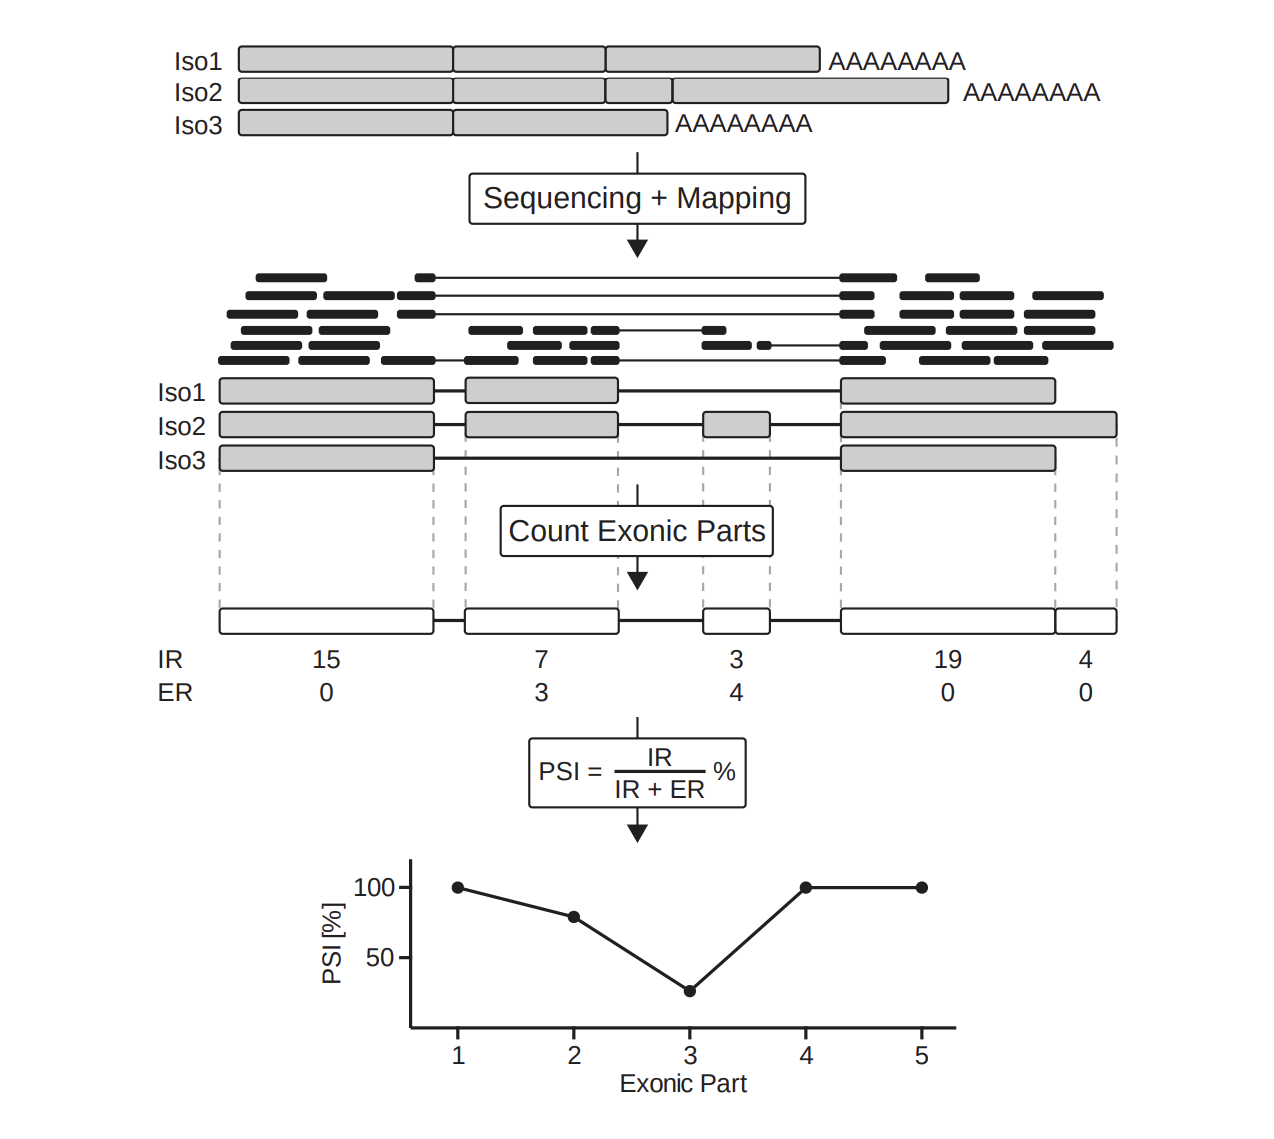
\includegraphics[width=0.7\textwidth]{../visualizations/ch4-methods/psi_estimation.png} 
	\caption{
		Process of estimating PSI based off RNA-seq reads \cite{berlinpsi}. The reads are mapped to the transcript. Based on annotation files, the reads overlapping exon/intron junctions are classfied as including or excluding reads for a particular exon. Based on the observed IR and ER, the PSI for a given exon is estimated.
		}
	\label{fig:psiestimation}
\end{figure}
%'deceptively simple'?

However, this estimate also has various issues:
\begin{enumerate}
	\item It doesn't account for uncertainty in the estimate. A rarely expressed gene may only experience a few reads of a particular exon leading to a very uncertain estimate. For instance, if we observe 1 IR and 1 ER for exon E1: $PSI_{E1} = \frac{1}{2} = 50\%$. Compare this to E2 where we observed 15 inclusion and 15 exclusion reads: $PSI_{E2} = \frac{15}{30} = 50\%$.\\
	The estimate of $PSI_E2$ is likely to be more accurate, but this information is not contained in the estimate. Concretely, these two samples would be treated as equally important by the network even though they likely shouldn't.
	
	One further processing step could be to only count exons who experienced at least a certain number of reads. However, assuming this solution is taken, there are additional two aspects worth discussing:
%	However, Assuming that one obtains a read count normalized by the gene expressiveness, there are two further aspects worth discussing:
%	\begin{enumerate}
%		\item This threshold soluton only alleviates this problem because one needs to account for the expressiveness of each gene: 10 reads in a lowly expressed gene may be as significant as 20 reads in a highly expressed gene. There are several measures for the expressiveness of a gene: Reads Per Kilobase Million (RPKM), Fragments Per Kilobase Million (FPKM) and Transcripts Per Kilobase Million (TPM). Of these, TPM is usually the most common choice. 
%		\item There is not a principled way to choose the cutoff threshold. The choice between a threshold which e.g. filters 5\% or 20\% of the samples is a trade-off between data quality and training samples. In practice, the optimal way to choose the cutoff threshold will be unknown and vary from dataset to dataset.
%	\end{enumerate}
	% https://www.rna-seqblog.com/rpkm-fpkm-and-tpm-clearly-explained/


	
	
	\item Reads which align purely to the flanking constitutive exons are ignored. While these could have occurred in either isoform, they provide latent evidence for whether the cassette exon was included or not. In isoforms where it occurred, the total length of the isoform is longer which means the reads are distributed over a larger area. This leads to a comparatively reduced proportion of reads across the flanking exons when the exon was included and vice versa. The estimate neglects to take this information into account.
%	This estimate ignores reads that align to the bodies of the flanking constitutive exons, which could have derived from either isoform. Nevertheless, these constitutive reads contain latent information about the splicing of the alternative exon, as higher expression of the exclusion isoform will generally increase the density of reads in the flanking exons relative to the alternative exon, and lower expression of the exclusion isoform will decrease this ratio of densities.
%	[MISO]
%	this is the reason why I wanted access to raw RNA-seq reads
	\item Related to 1), typically multiple samples or biological replicates of a given experiment are available. It is desirable that reads across multiple samples can be integrated to give a more well-adjusted estimate. How to best achieve this is not obvious. Read depths between multiple libraries may vary and this should be accounted for. [possible other issues here and then make this another itemization]
	\item IR and ER must be normalized for exon length to obtain meaningful results. For a long exon, the majority of reads will be IR because they can be located over a much larger area than the ER who must overlap with the 0-length feature of the splicing junction. This can be accounted for by normalizing for the possible number of start positions for each read population:
	$$\#IR_{norm} = \frac{\#IR}{exon\_length + read\_length -1}$$
	$$\#ER_{norm} = \frac{\#ER}{read\_length - 1}$$
	%TODO: check out second graphic from berlin paper in more detail
%	Note that this assumes that reads are uniformly distributed across a transcript isoform. It is well-known that RNA-seq reads are biased .... [get paper from Liz/Wilfred]
	
	%	thought: this normalization doesn't obviously seem correct to me on second thought. an ER can be found at two junctions, so that would double the number of possible read starts
	%	IR can only start from position 0 to exon.length-read.length of the exon can't they?
	%	won't do anything about this, but will want to use weaker claim
	%	I think you can't really do normalization for junction counting

%	The goal of these adjustments is not to arrive at perfect estimates, but rather to alleviate the influence of systematic biases as much as possible. 
	
	%: could add that even then reads across a gene aren't evenly distributed
	% see https://bmcbioinformatics.biomedcentral.com/articles/10.1186/1471-2105-12-290
	
	\item Reads may be misattributed. The motivation for analyzing splicing at a level of alternative splicing events is that full gene isoforms can not reliably be quantified given the currently available short RNA-seq read lengths. However, this issue may still occur at the splicing event level when two splicing variants of an exon share a junction. This is illustrated in Figure \ref{fig:misattribution}.
	This misattribution of a read can only be corrected by considering circumstantial evidence, similar to 2.; for instance, read counts on the exon junction may give evidence regarding to which splicing event the read at the shared junction belongs.
\end{enumerate}

\begin{figure}
	\centering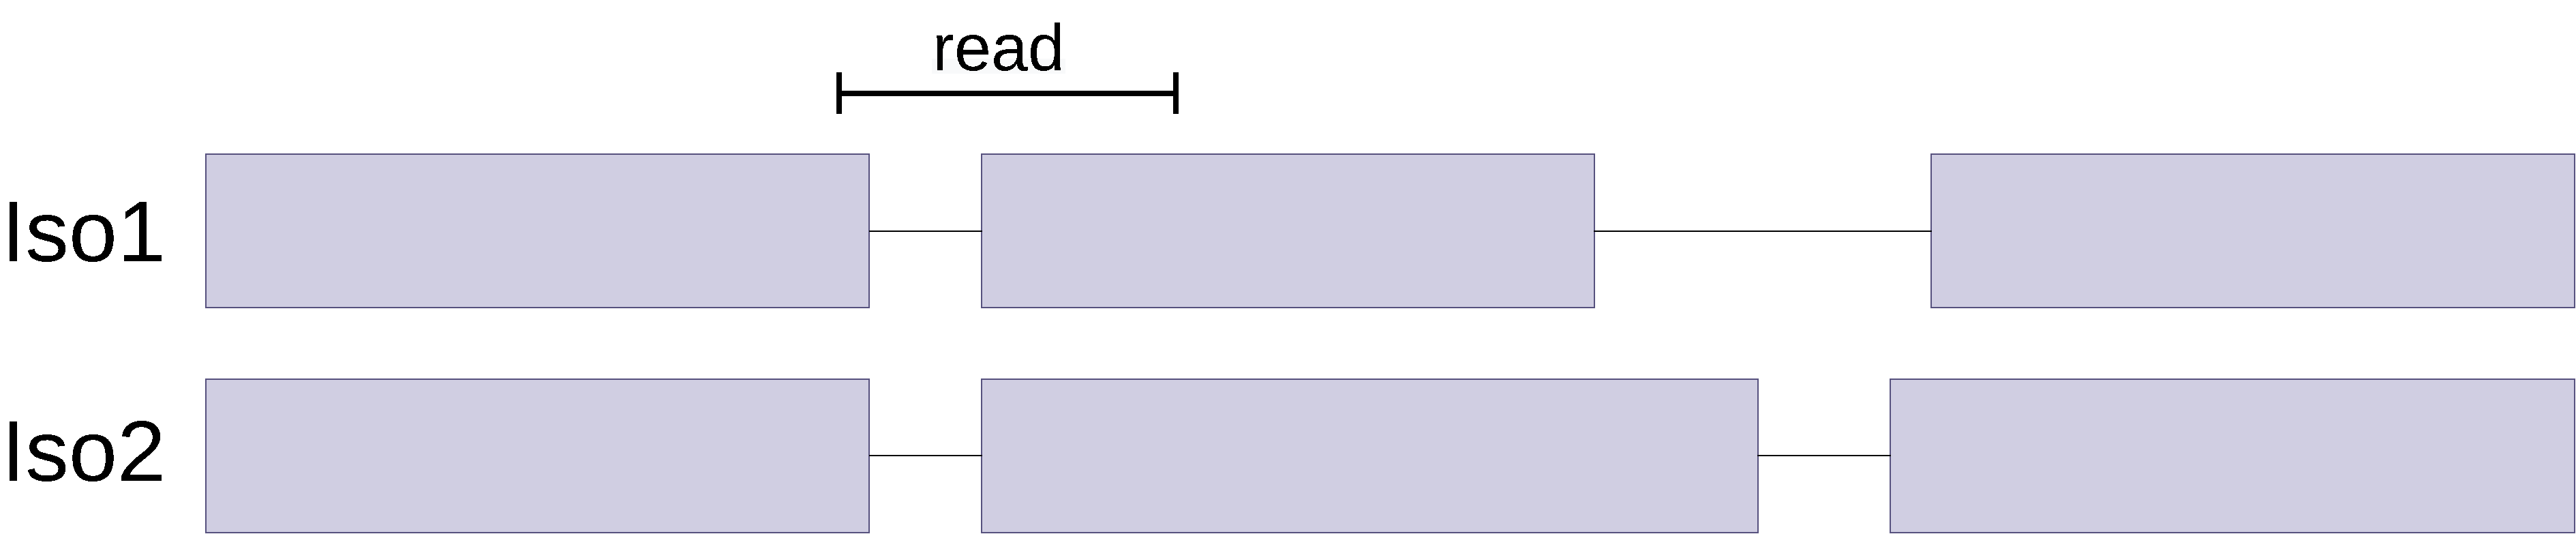
\includegraphics[width=0.7\textwidth]{../visualizations/ch4-methods/visualizations-misattribution.pdf} 
	\caption{The read across the exon-exon boundaries may be attributed to isoform 1 or isoform 2. Consequently, it may also be attributed to the first or second splicing variant of the middle exon.}
	\label{fig:misattribution}
\end{figure}

%hopefully was able to demonstrate that this estimate is problematic and may easily be unreliable.
Due to these issues relating to calibrating for uncertainty, to not making use of all of the available evidence, to integrating reads across multiple samples and misattributing reads, this estimate is problematic.

\subsubsection{A word of caution} \label{subsubsec:caution}
Even if all of these issues are perfectly handled, the resulting estimate would still not be perfect. For instance, the 'solutions' for 1. and 4. implicitly rely on the assumption that reads across a transcript are evenly distributed. It is well-known that sequence reads across a transcript aren't equally distributed due to biases relating to GC-content \cite{gccontentbias}, gene length and dinucleotide frequencies \cite{rnaseqbiascorrection}.
% or transcript length bias. 
 % there is also transcript length bias, see https://biologydirect.biomedcentral.com/articles/10.1186/1745-6150-4-14
 % but this bias is more about biases between transcripts rather than within a given transcript
 %[ list of biases duplicate reads, stacking reads]. 
% : stashed for now; https://bmcbioinformatics.biomedcentral.com/articles/10.1186/1471-2105-12-290
% https://www.the-scientist.com/news-opinion/technical-bias-widespread-in-rna-seq-datasets-66766#:~:text=Love%20adds%20that%20there%20are,length%2Drelated%20biases%20as%20well.
% https://emea.support.illumina.com/bulletins/2017/04/considerations-for-rna-seq-read-length-and-coverage-.html#:~:text=Experiments%20looking%20for%20a%20more,for%20mRNA%2Fwhole%20transcriptome%20sequencing.
%https://genomebiology.biomedcentral.com/articles/10.1186/s13059-016-0881-8
These biases are not easily quantifiable and can never be perfectly corrected for.\\
%and even already adjusted read estimates (e.g. for gene expressiveness) are still biased. \\
In more general terms, the data on which the estimate is based is inherently very noisy and this will always lead to downstream effects independent of the preprocessing method used. The question is not whether the resulting estimate is still biased, but rather if the effect of systematic biases influencing it can be alleviated enough for the estimate to be useful. 
%TODO i basicallly say here that unbiasing rna-seq data will never be possible - opinions from wil and liz? lol
\subsubsection{Dataset based on HEXEvent}
% https://www.ncbi.nlm.nih.gov/pmc/articles/PMC1431573/
The HEXEvent database already provides PSI estimates based on EST counts for each exon and facilitates standard filtering steps (e.g. only select cassette exons). 
The baseline paper \cite{dsc} takes HEXEvent as a starting point and generates three different datasets respectively only containing cassette exons, exons with an alternative 3' splice and exons with an alternative 5' splice site. Each of these datasets also contains constitutive exons. To account for the biases inherent in EST data, it applies multiple filtering steps such as requiring a minimum number of supporting ESTs and only using exons which display a single type of alternative splicing. They make the resulting datasets publicly available and we use the dataset containing cassette exons for direct comparability. 

% TODO: color models
However, it should be noted that HEXEvent uses the critized naive estimation method for PSI, i.e., they estimate PSI as $PSI = \frac{\#IR}{(\#IR+\#ER)}$. They don't explicitly account for any of the four main critique points discussed above. The EST data available by UCSC is based on many different tissues which may lead to the derived alternative splicing behaviour being an average of the splicing behaviour of many tissues which never occurs in any singular tissue. %distort view, confuse nice words here
Therefore, care should be taken when drawing conclusions based on the PSI estimates of this dataset. 

\subsubsection{Our PSI estimation implementation} \label{subsubsec:implementedpsiestimation}
To obtain a PSI estimate based on the publicly accessible exon-exon junction read counts of the GTEx project, we implement our own PSI estimation method. We are not able to use the published methods we introduce below, as they require access to the raw RNA-seq reads which we don't have access to due to data privacy regulations.

GTEx gives access to data based on sample from different tissue. It also gives access to information about which sample types were taken from which donor (in an anonymized way). We use this information to find a donor from whom brain cortex tissue, cerebellum tissue and heart tissue samples were taken. For each sample we derive two datasets: one exon-centric dataset which only consists of cassette exons and one intron-centric dataset which consists of every junction found in the original data.
We obtain six datasets in total.

Fundamentally, our estimation relies on the formula $PSI = \frac{\#IR}{(\#IR+\#ER)}$. However, before computing PSI, we also apply the following filtering and normalization steps:
%\begin{itemize}
%	\item cassette exons which are shorter than 25 nt and introns which are shorter than 80 nt are excluded. Exon and intron of these lengths constitute less than 1\% of exons and introns in total and are usually caused by sequencing errors \cite{dsc}.
%	\item GTEx provides access to TPM values for each gene from a sample. Adressing point 1. from \ref{subsubsec:naivepsi}, we obtain the TPM-adjusted read counts via $\#IR^{TPM} = \frac{\#IR\}{TPM}$ and $\#ER^{TPM} = \frac{\#ER\}{TPM}$. To address spurious reads from lowly-transcribed genes having a disproportionate impact, we only count reads from genes whose TPM is larger than 10. This is by far the most stringent filtering method we apply, leading to about two-thirds of genes being filtered. This cut-off was chosen so aggressively as data quality is paramount. More details are given in Figure %\ref{fig:tpm_distribution}.
%	\item Adressing point 4. about IRs naturally being more common than ER from \ref{subsubsec:naivepsi}, we estimate the read length of the RNA-seq reads to be 150 on average \cite{gtex_read_length} and apply the proposed normalization method: $\#IR^{TPM}_{norm} = \frac{\#IR^{TPM}}{(exon length + 149)}$ and $\#ER^{TPM}_{norm} = \frac{\#ER^{TPM}}{149}$.
%\end{itemize}

Using the normalized \#IR and \#ER of all exons and junctions remaining after filtering, we then compute PSI: $PSI = \frac{\#IR^{TPM}_{norm}}{(\#IR^{TPM}_{norm}+\#ER^{TPM}_{norm})}$. 

This estimate fails to take into account the information contained in non-junction reads, as we simply don't have access to them.
This estimate also does not aggregate the information from multiple biological samples, although we took care to choose the donor with tissue samples from brain cortex, cerebellum and heart, whose total read count was the highest. 
Reads may also be misattributed in our estimation as described in 5. of \ref{subsubsec:naivepsi}.
%The initial dataset contained roughly 10 million total exon-exon junction read count for each tissue distributed over roughly 330,000 unique junctions. More statistics about this dataset, and the others, are given in Section \ref{subsec:datasetstatistics}. 

%After the PSI values have been obtained as described above, we apply the final sample processing steps as described in \ref{subsec:finalsampleprocessing}.
%TODO tpm value histogram
%\begin{figure}
%	\centering%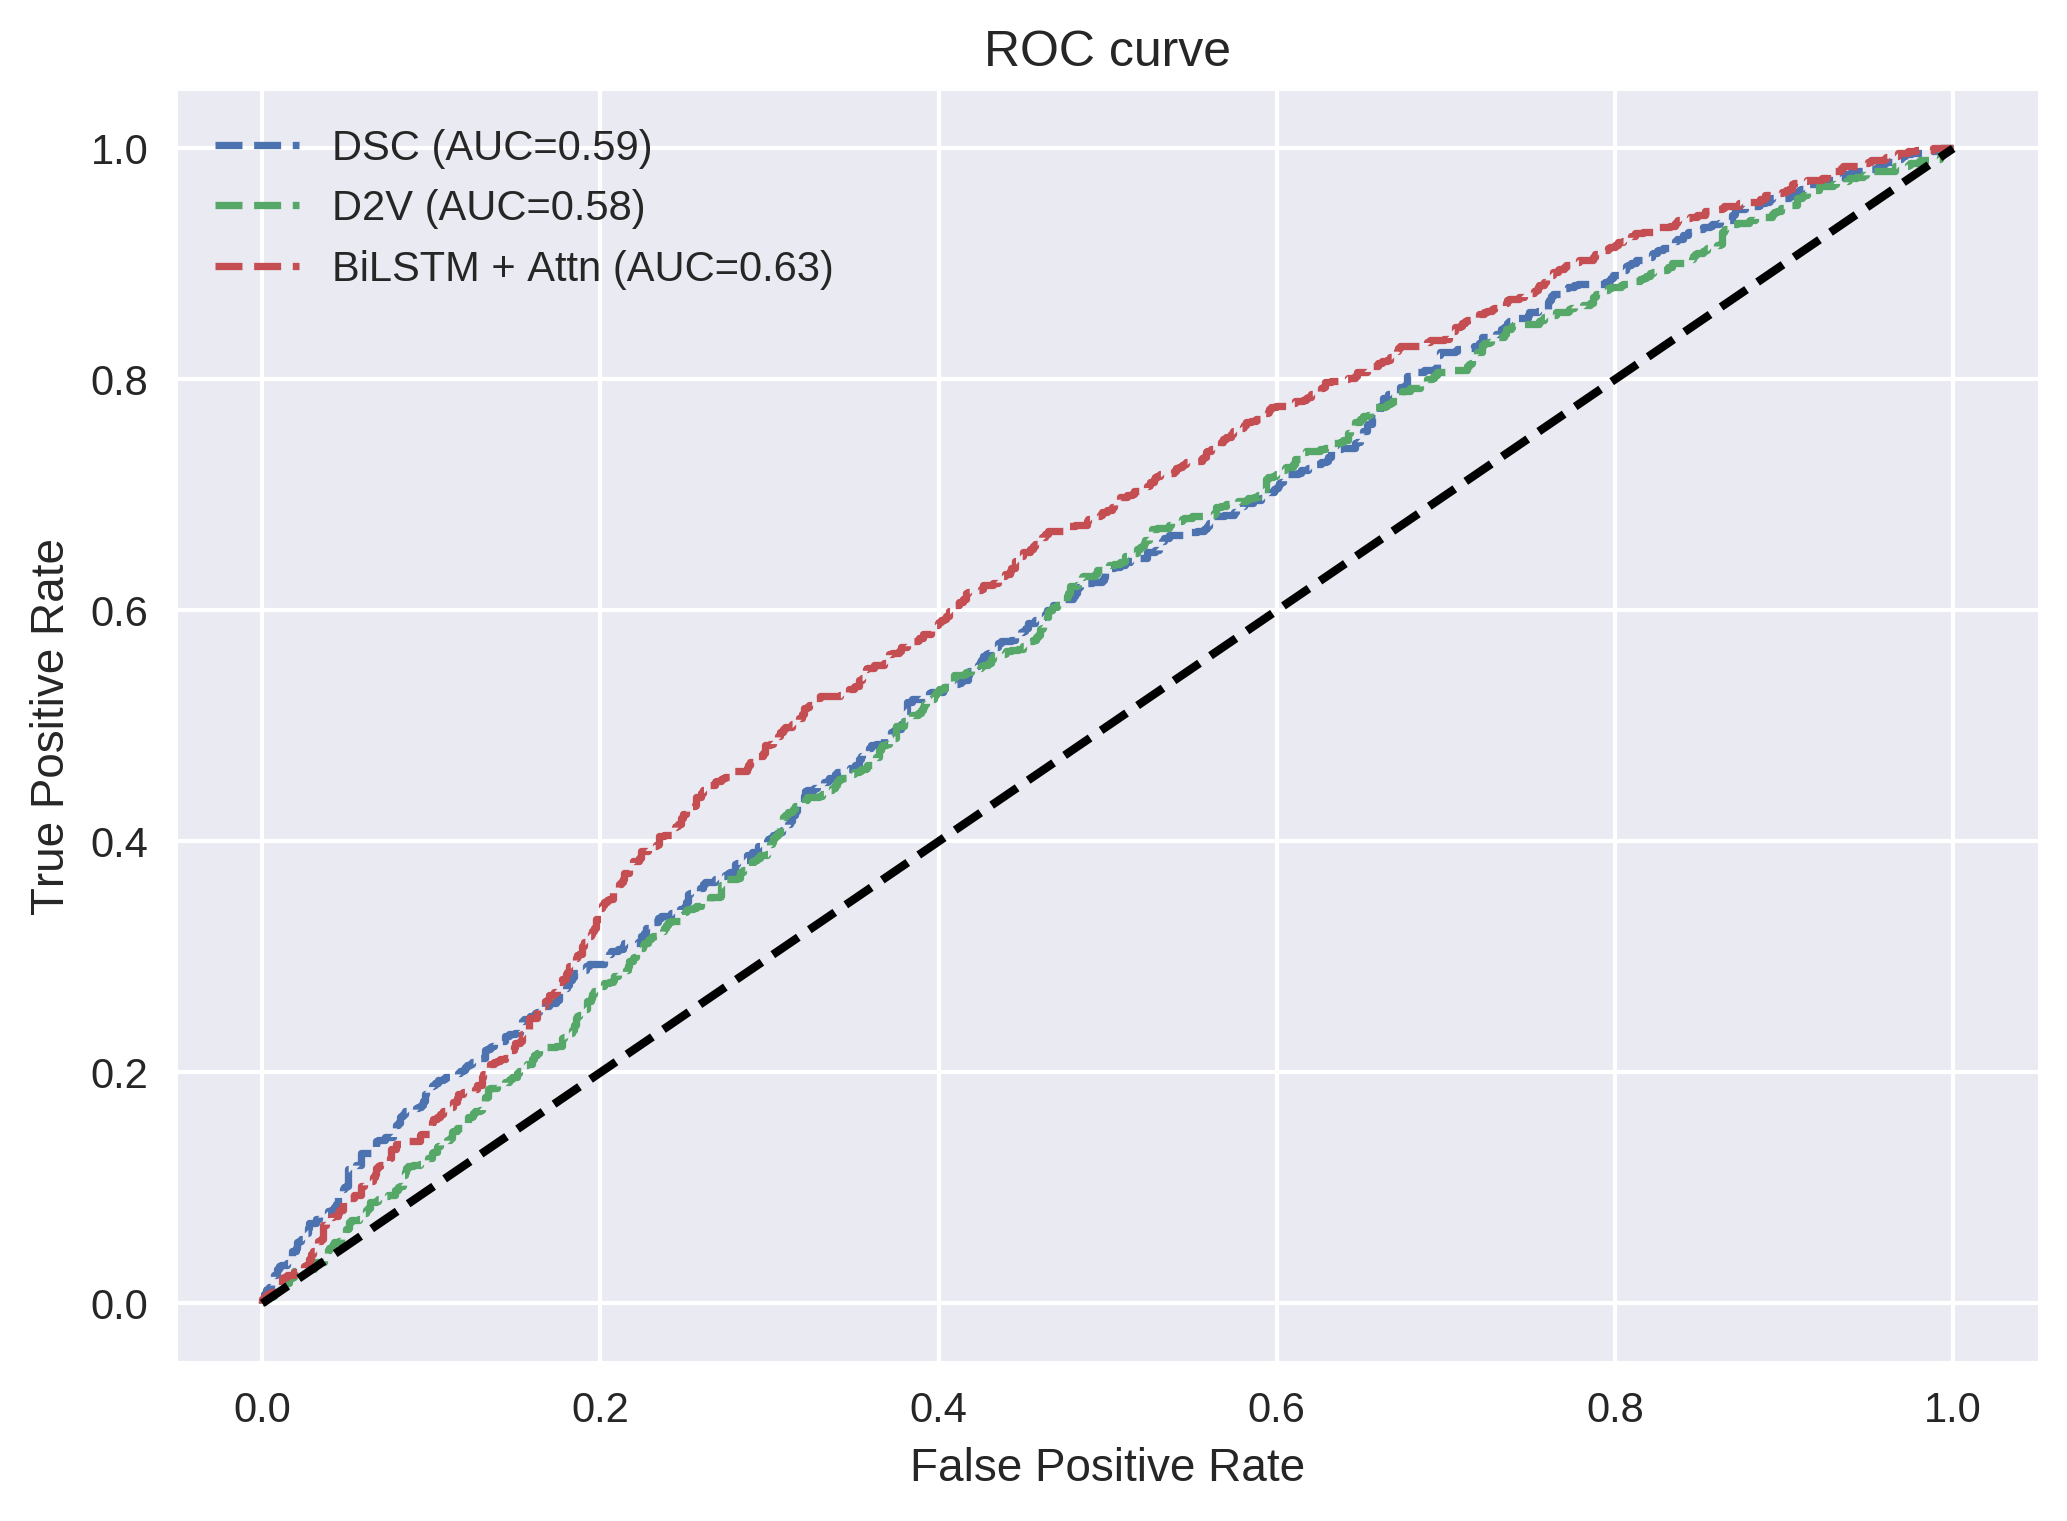
\includegraphics[width=0.7\textwidth]{../visualizations/suppa_cross_model_roc_auc_comparison.png} 
%	\caption{%TODO tpm value histogram
%		Distribution of TPM values. The cut-off we chose is marked in red. Concretely, this lead to filtering ... out of ... genes. }
%	\label{fig:tpm_distribution}
%\end{figure}
%1) TPM: Only take reads from genes across a certain TPM into account (because random spurios reads from low TPM genes could have an outsized effect on the estimation). Say that you weight reads according to the respective TPM. Show TPM distribution and say what TPM threshold you use.\\
%2) Latent information: Say how there is nothing you can do, due to only having access to the junction reads themselves. \\
%3) Multiple samples: Unclear how to best do this and skipped for now. However, basing estimatin based on the sample with the maximum total amount of reads. \\
%4) Start pos normalization: Say that you estimate read length to be 150 and do this. \\
% TODO: mention junction datasets
% potentially even more details; eg how you use this heuristic of checking the 10 samples past the current one
% todo add details such as exact name of individuals used and number of reads
% TODO add this information in appendix bezi1, bezi2, lexy2 and sample number 1 with ERR number .... 




\subsubsection{More sophisticated PSI estimation approaches}

Several approaches have been developed which try to address the issues in estimating PSI. However, many of these focus purely on the differential splicing changes between conditions (in the form of delta PSI) and don't directly report the PSI in a given condition which is what we are initially interested in. Of the methods directly reporting PSI, we chose the two fast methods SUPPA and MAJIQ. SUPPA and MAJIQ represent two different approaches to PSI estimation: SUPPA is primarily based on quantification of transcripts, while MAJIQ is based on building up a splicing graph. Figure \ref{fig:dataset_creation_process} shows the high-level steps taken when using MAJIQ and SUPPA to create datasets for training.



\begin{figure}
	\centering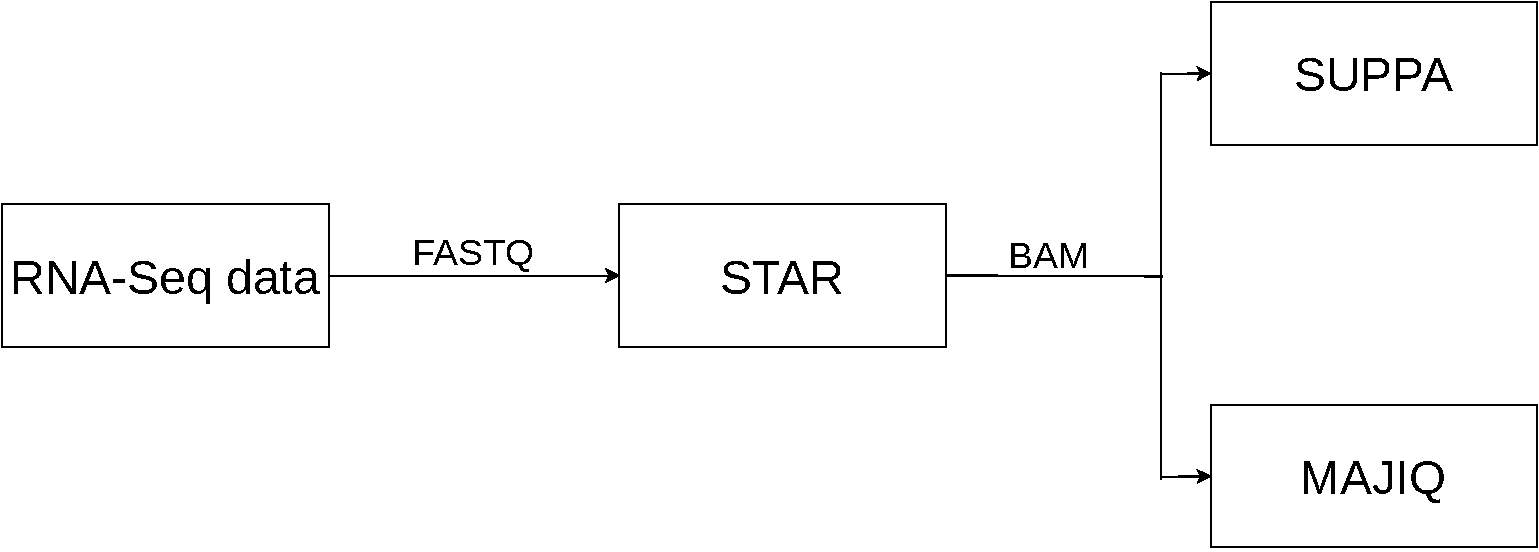
\includegraphics[width=0.7\textwidth]{figures/d2v-Page-3.pdf} 
	\caption{Data flow when using MAJIQ or SUPPA to create a training dataset. }
	\label{fig:dataset_creation_process}
\end{figure}
%isoform-based vs count-based methods
%	count-based methods = exon based and event-based methods
\subsubsection{SUPPA}\label{subsubsec:suppa}
SUPPA2 \cite{suppa2} estimates the PSI value for each alternative splicing event based on transcript abundances. It operates in 2 steps for quantifying the PSI of an alternative splicing event:
1) Given an input annotation file in GTF format, it generates the transcript isoforms which count as IR or ER for a given alternative splicing event.
2) Given the information which transcript count as IR or ER from 1) and how frequently each transcript occurs, it estimates the PSI value via $PSI = \frac{TPM_{IR}}{TPM_{IR} + TPM_{ER}}$. SUPPA2 can integrate the TPM values from multiple samples.
%because it is so naive is probably the reason why it performs so badly
%!perhaps add steps 1/2/3 to this graphic?


\textbf{Using SUPPA2:}
SUPPA2 requires a GTF annotation file and a file quantifying the abundance of each transcript. A GENCODE version 34 annotation file obtained from Ensembl was used as an annotation file. Salmon was used for quantifying the relative abundance of each transcript in TPM. Salmon's [cite] quantification is based on the raw RNA-seq reads in FASTQ format, takes into account experimental attributes and correct for biases commonly observed in RNA-seq data. After extracting the TPM values provided by Salmon into the format required by SUPPA (a tsv-file with one column for the transcript id and one column for the TPM value), SUPPA2 estimates the PSI for each alternative splicing event.
The latest version of SUPPA available as of July 2020 was used (SUPPA v2.3). 
%[https://github.com/comprna/SUPPA/releases/tag/v2.3 if I feel like it]
\subsubsection{MAJIQ}\label{subsubsec:majiq}
Modeling Alternative Junction Inclusion Quantification (MAJIQ) builds up a splice graph \cite{majiq2} which contains exon as vertices and junctions as edges. An edge is added between two vertices if a transcript isoform is found in which they share a junction (that is if the exons are neighbours and everything between them has been spliced out).
Constitutive exons are vertices with two incoming edges.
Vertices which have more than 3 incoming edges are denoted as local splicing variations (LSV). Due to this problem formulation, MAJIQ can model more complex splicing variations than skipped exons, alternative 3' splice sites, and alternative 5' splice sites. Figure \ref{fig:splice_graph} shows an example splice graph. Importantly, apart from estimating $\delta$ PSI between different conditions, MAJIQ is also able to directly estimate PSI for a given condition. The estimation is done using a combination of read rate modelling, Bayesian PSI modelling and bootstrapping. The only issue from \ref{subsubsec:naivepsi} MAJIQ doesn't account for is 2.: the integration of the information from non-junction reads. 
% looked at mjiq paper; it only seems to look at juntons
% hadnles eg point 5. by only looking at junctions until the very end and modelling eg cassette exons as two distinct LSVs --- ie each junction will have its own PSI


\begin{figure}
	\centering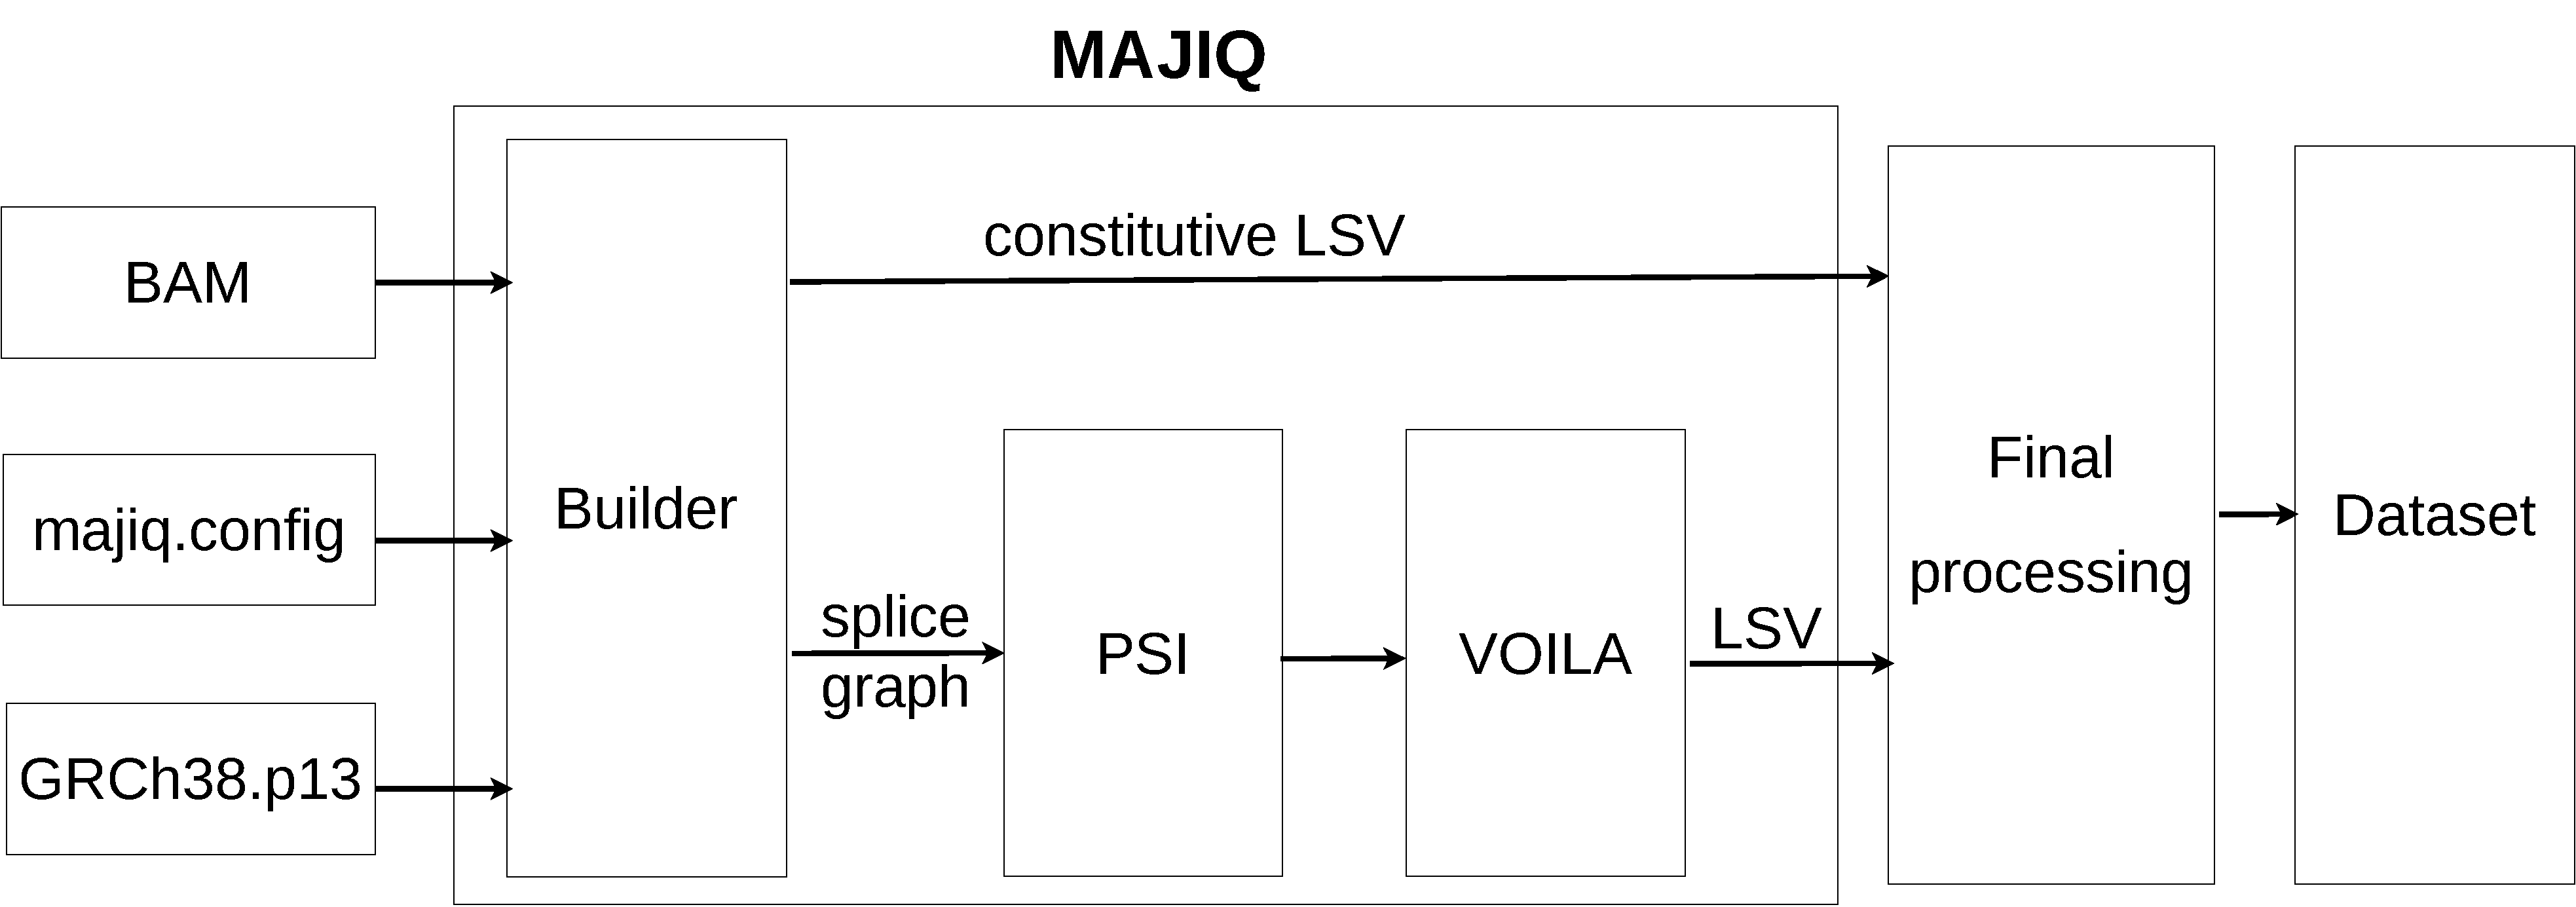
\includegraphics[width=0.7\textwidth]{figures/d2v-majiq.pdf} 
	\caption{Data flow when using MAJIQ to create a training dataset. }
	\label{fig:majiq_dataset_creation_process}
\end{figure}

\begin{figure}
	\centering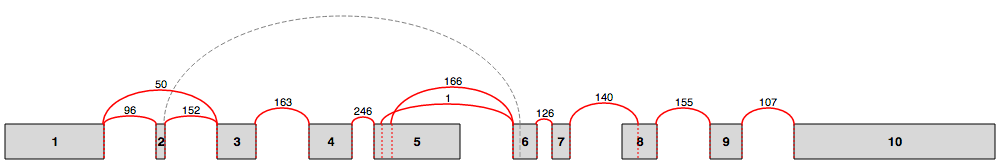
\includegraphics[width=0.7\textwidth]{../visualizations/ch4-methods/splice_graph.png} 
	\caption{An example splice graph as displayed in VOILA \cite{majiq2}. Exons, represented by grey rectangles, are connected with another exon via an edge, if a junction between the exons (or a variant of them) is observed. The number above an edge displays the number of observed raw reads spanning a particular exon-exon junction.}
	\label{fig:splice_graph}
\end{figure}

\textbf{Using MAJIQ:} MAJIQ requires sequence files in bam format (along with their respective index files) and an annotation DB in gff3 format. The bam format is a format for aligned RNA-seq reads. 
To this end, the raw reads from each sample were uploaded to the bioinformatics data processing platform Galaxy \cite{galaxy} from the European Nucleotide Archive (ENA). For each sample, the raw reads in FASTQ format were then mapped to the RNA using STAR \cite{star}. STAR produces the required bam and bai format files as output.

The required gff3 file used is human GRCh38 release 13.
MAJIQ use then proceeds in three stages. First MAJIQ Builder takes a configuration file, the gff3 annotation and the bam and bai files of all samples as input and builds up the splicing graph. At this stage, MAJIQ also identifies constitutive exons and optionally dumps them to a file. This option was used.
Secondly, MAJIQ PSI estimates the PSI of the LSV candidates obtained through MAJIQ Builder. MAJIQ PSI improves the accuracy of its PSI estimate by integrating evidence across multiple samples.
Finally, the obtained LSVs can be visualized using VOILA. VOILA also allows filtering of LSV according to type. See Figure \ref{fig:voilaexample} for an example output of VOILA. For this study, only LSV which denoted exon skipping were used. The filtered LSV along with the constitutive exons obtained from MAJIQ Builder were then used for processing as described in Section \ref{subsec:finalsampleprocessing}.\\
The latest version of MAJIQ available as of July 2020 was used (MAJIQ v2.0).


\begin{figure}
	\centering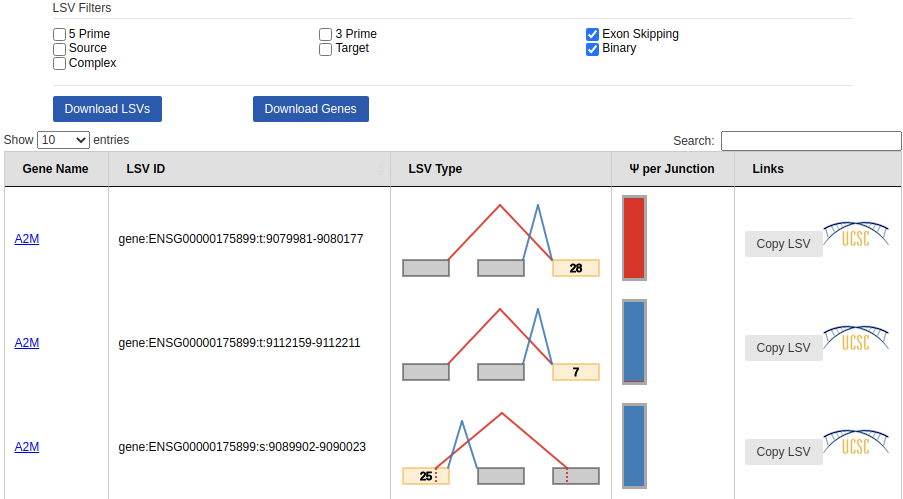
\includegraphics[width=0.7\textwidth]{../visualizations/ch4-methods/voila_example.png} 
	\caption[Four-chamber illustration of the human heart.]{Example output of VOILA while filtering for LSV which only experience exon skipping and no other alternative splicing event. }
	\label{fig:voilaexample}
\end{figure}


The naive way of estimating PSI was applied to the GTEx dataset as we had no access to raw RNA-seq reads and couldn't apply SUPPA nor MAJIQ. SUPPA and MAJIQ were applied to the data from the HipSci repository.
\subsection{Final sample processing} \label{subsec:finalsampleprocessing}

\begin{figure}
	\centering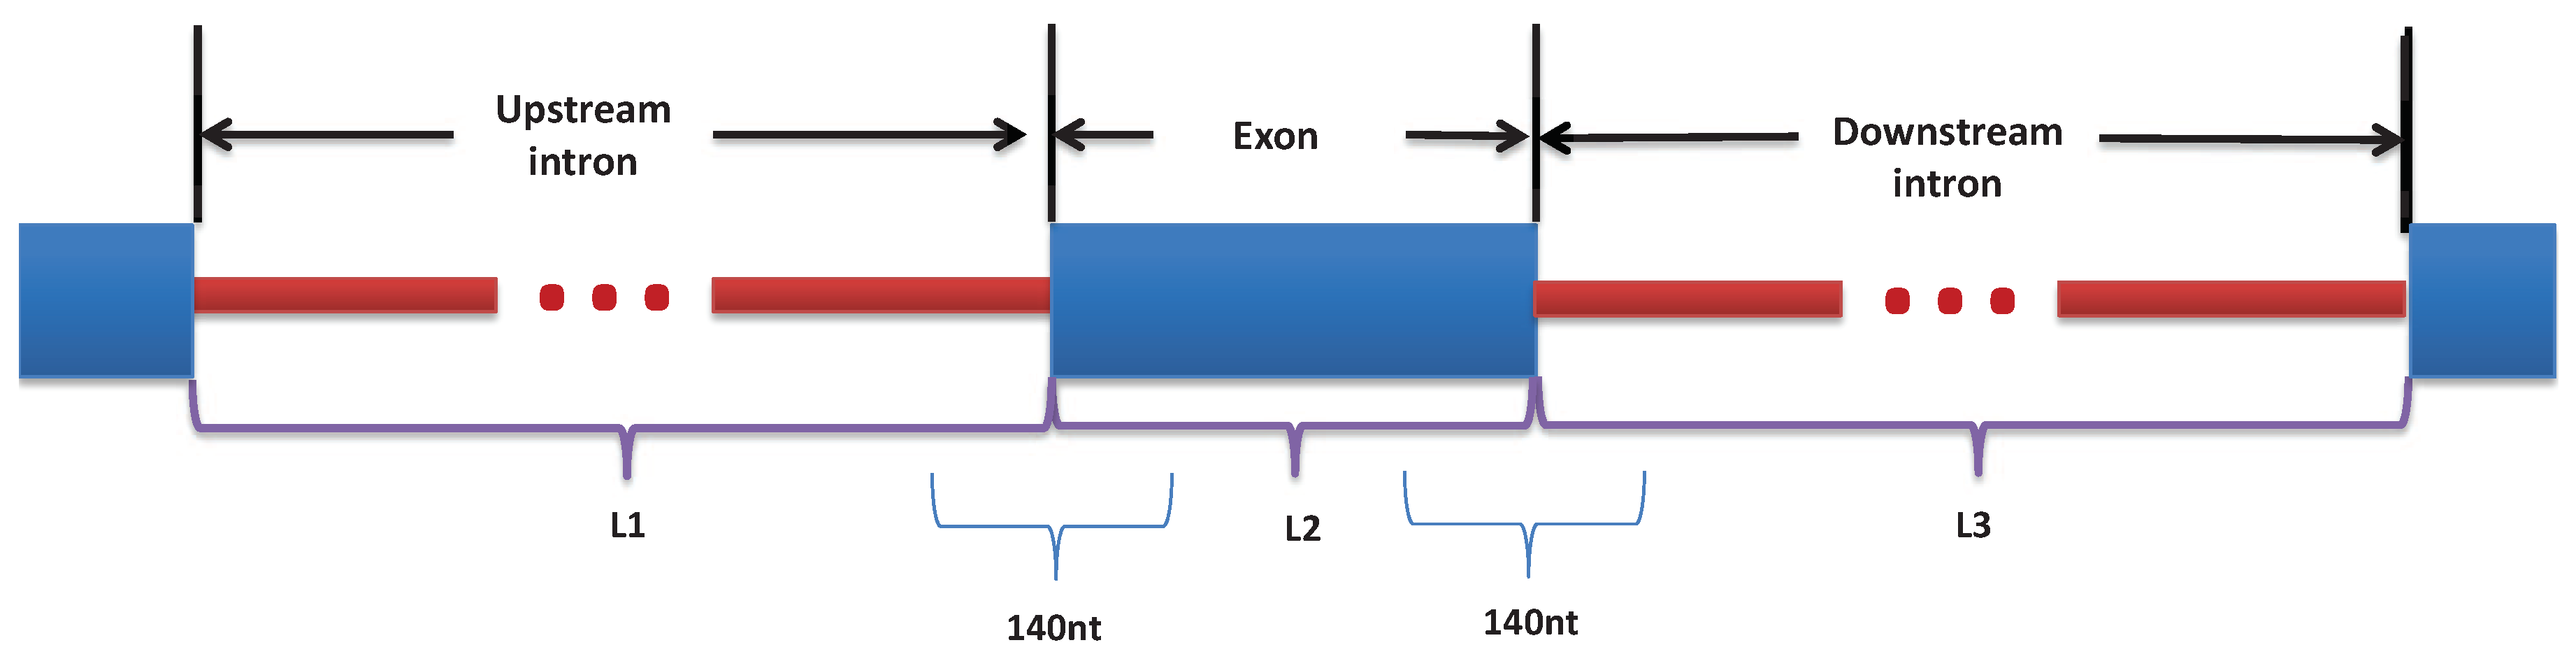
\includegraphics[width=0.7\textwidth]{../visualizations/ch4-methods/input_schematic.png} 
	\caption[bla.]{Schematic of model input \cite{dsc}. The input are the 140 nucleotide region extracted around the exon start and exon end, as well as the normalized length of the exon and its flanking introns. }
	\label{fig:inputschematic}
\end{figure}

Using the output of the previous preprocessing steps, now either exon-centric or intron-centric samples are created. Exon-centric samples are created when the task of the network is to classify an exon as constitutive or not. Intron-centric samples are created when the task of the network is to classify whether a junction is constitutive or not.
At this point, the datasets have been preprocessed that each sample at least contains the following:

\begin{itemize}
	\item chromosome and strand information of the to-be-classified exon or junction,
	\item start and end coordinates of the exon or junction within a chromosome,
	\item the lengths of neighbouring introns or exons.
\end{itemize}

Using the chromosome information and the start and end coordinates, a 140 nucleotide window around the start and end coordinates are extracted (see Figure \ref{fig:inputschematic}). Furthermore, if an exon or junction is taken from a negative strand, the extracted start and end windows are switched, the order of the nucleotides within the start and end windows are reversed and each extracted nucleotides is converted to its reverse complement. This way the models don't have to learn different features for exons or junctions on the + and - strand.
Samples from the chromosomes X, Y and M were excluded due to the fundamental functional differences between them and the autosomes. \\
The extracted nucleotides were one-hot encoded as four dimensional vectors. Specifically, adenine 'A' was encoded as [1 0 0 0], cytosine 'C' as [0 1 0 0], guanine 'G' as [0 0 1 0] and thymine 'T' as [0 0 0 1]. Thus each 140 nucleotide long window was converted into an 140x4 matrix containing one-hot encodings.

It is commonplace that repetitive sequences are soft-masked as lower case letters in the reference genome. As this has no known bearing on alternative splicing, this information was ignored during one-hot encoding.

As in previous work \cite{dsc} \cite{flawed4}, we include the exon and intron lengths as input feature. This was motivated by the observation that exon and intron lengths are correlated with splicing behaviour \cite{lengthsref1} \cite{lengthsref2}. In particular, alternatively spliced exons tend to be flanked by longer introns. This may be due to long intronic sequences making it more challenging for the spliceosome to locate the exon or it plainly being more likely that novel exons originate within long introns \cite{bestlengthsref}. 

%In addition to sequence information, the lengths of neighbouring introns or exons, as well as the length of the exon itself, are given as input to the models. Several studies have shown that exon and intron lengths can influence splice-site recognition. [15,34] In addition, previous studies have shown that including the length information dramatically model performance. [DSC] 

Introns are on average one to two orders of magnitudes larger than exons and their relative standard deviation is three times as large as that of exons. To avoid giving features to the network whose magnitude might differ by several orders of magnitude, the intron and exon lengths features were respectively normalized through the mean length and standard deviations of internal exon ($\mu=145, \sigma=198$) and introns ($\mu=5340, \sigma=17000$) in the human genome (see Appendix \ref{app:lengths}). For brevity, the normalized intron and exon lengths given to the network are often referred to as the length features.

In some of the datasets the number of constitutive and non-constitutive samples are not very evenly divided. For instance, the HexEvent dataset contains roughly times three as many constitutive as alternatively spliced samples. This leads to the issues with models getting stuck in local minima where they just predict the majority class. This was alleviated by including each alternatively spliced sample multiple times until the classes were balanced.

A single sample input to the model contains two 140x4 one-hot encoded matrixes and three normalized length values. The associated ground truth with each sample is the scalar 1 if the respective exon or junction is constitutive, and 0 if not.
\subsection{Dataset statistics} \label{subsec:datasetstatistics}

%TODO: Table [in overleaf atm] shows the absolutes number of obtained training samples for all datasets which were used.
% TODO add more statistics now; decision to show the junction results (as majiq also does modelling predominatly on junctions), as i can say that my gtex dataset will have constitutive junctions and no issue with misattributed reads
further analysis postponed until I ran experiments again and decided for which datasets I will show results 

%hexevent:
%Total number of exons: 50918
%Number of low PSI exons: 39128
%Number of high PSI exons: 4952
%Number of cons exons: 6838
%gtex exon brain
%Number of generated training samples: 32682
%Number of low PSI exons: 15872
%Number of high PSI exons: 7961
%Number of cons exons: 8849
%gtex exon cerebellum
%Number of generated training samples: 39874
%Number of low PSI exons: 19355
%Number of high PSI exons: 6791
%Number of cons exons: 13728
%gtex exon heart
%Number of generated training samples: 20806
%Number of low PSI exons: 9569
%Number of high PSI exons: 5216
%Number of cons exons: 6021
%gtex junction brain
%Number of generated training samples: 127908
%Number of low PSI exons: 58560
%Number of high PSI exons: 14538
%Number of cons exons: 54810
%gtex junction heart
%Number of generated training samples: 81659
%Number of low PSI exons: 36354
%Number of high PSI exons: 9389
%Number of cons exons: 35916
%gtex junction cerebellum
%Number of generated training samples: 161310
%Number of low PSI exons: 74139
%Number of high PSI exons: 13151
%Number of cons exons: 74020
%gtex reconstruction junc (brain)
%Number of skipped non-DSC junctions: 71868
%Number of low PSI junctions: 23943
%Number of high PSI junctions: 7281
%Number of cons junctions: 25977
%Total number of junctions: 57201
%gtex reconstruction exon (brain)
%Number of low PSI exons: 3458
%Number of high PSI exons: 1989
%Number of cons exons: 23505
%Total number of exons: 28952
%hipsci majiq junc (neuron)
%total: 90627
%Number of cons junctions: 48163
%Number of alt juncs: 42464 (from 21232 exons)
%Number of low PSI exons: 22834
%Number of high PSI exons: 19630
%hipsci majiq exon (neuron)
%total: 44746
%Number of cons exon: 26394
%Number of alt exons: 18352
%Number of low PSI exons: 8201
%Number of high PSI exons: 10151
%hipsci suppa exon (neuron)
%Number of samples: 17863
%Number of low PSI exons: 9828
%Number of high PSI exons: 311
%Number of cons exons: 7724
%hipsci majiq exon (iPSC)
%total: 48489
%Number of cons exon: 27371
%Number of generated training samples: 21118
%Number of low PSI exons: 9299
%Number of high PSI exons: 11819
%some analysis of the numbers, e.g. junction datasets way larger
%probably won't include reconexon/junction dataset

%gtex number of reads:
%The initial dataset contained roughly 10 million total exon-exon junction read count for each tissue distributed over roughly 330,000 unique junctions.

\begin{figure}
	\centering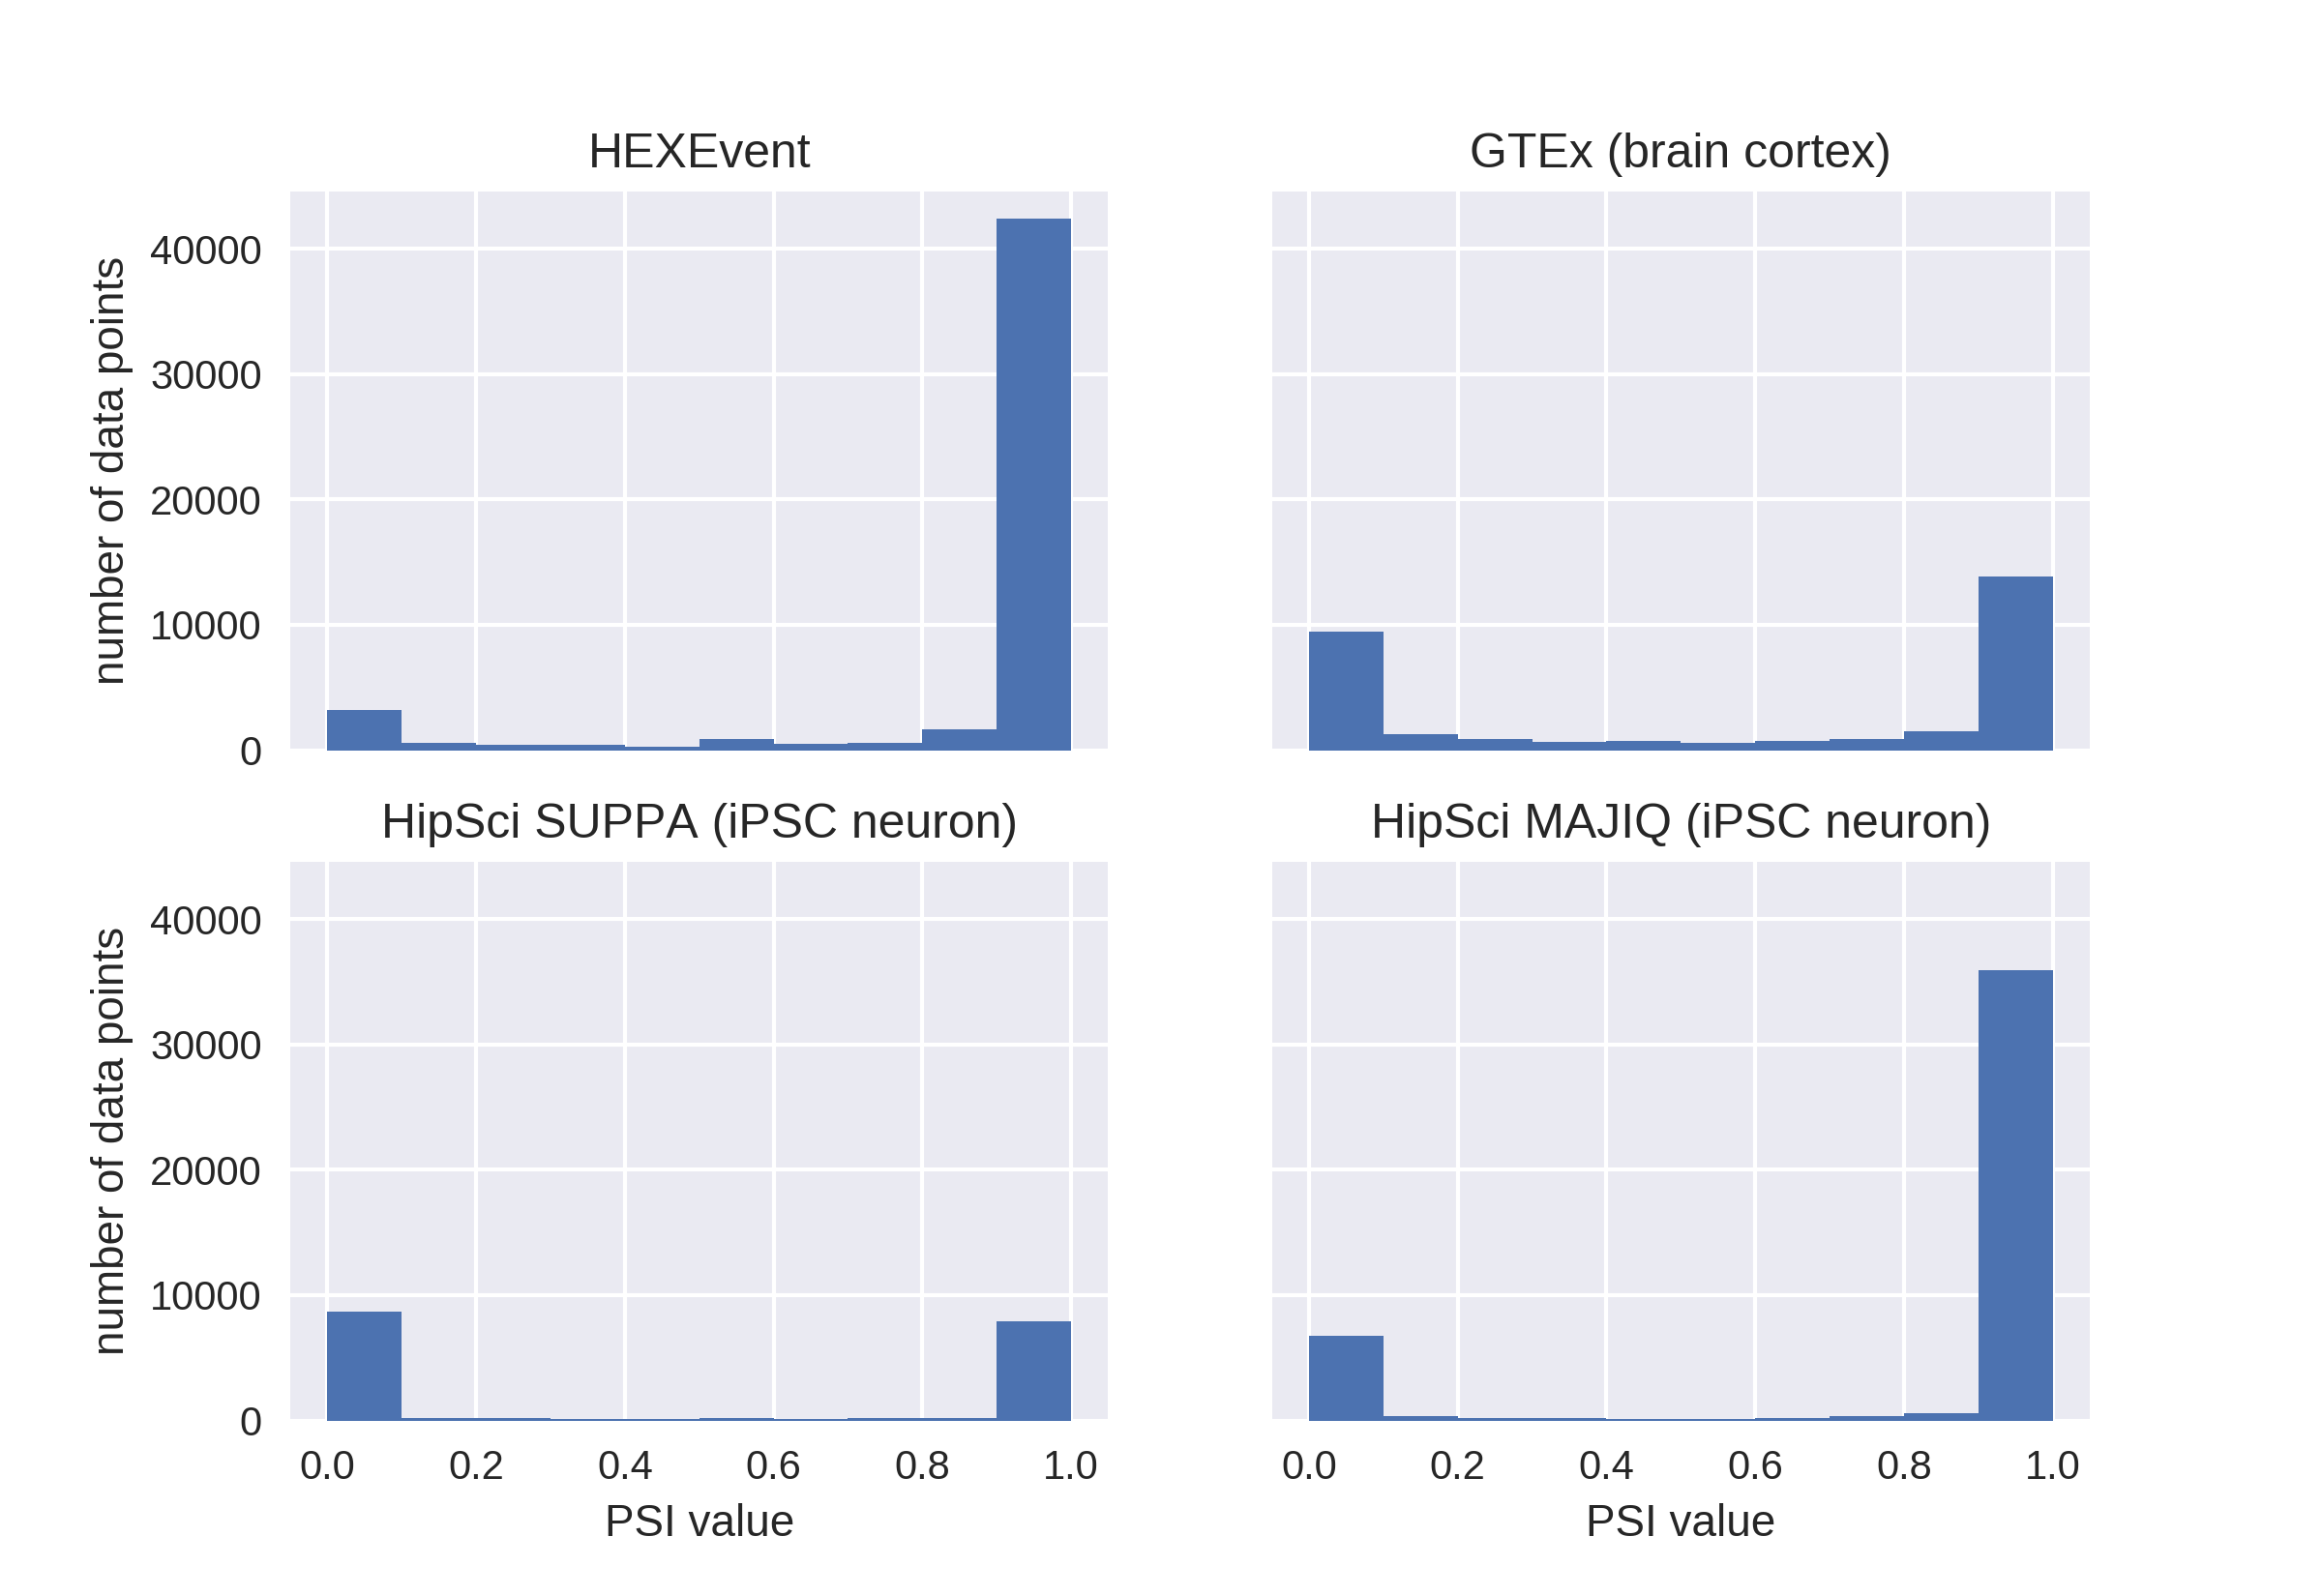
\includegraphics[width=0.7\textwidth]{../visualizations/ch4-methods/dataset_histograms_seaborn.png} 
	\caption[test.]{
		Histograms comparing the exon-centric versions of the four fundamentally different training datasets used. The shown GTEx dataset is based on samples from brain cortex tissue and  the shown HipSci datasets are based on samples from iPSC cells differentiated to neurons. 
	}
	\label{fig:datahistograms}
\end{figure}

Figure \ref{fig:datahistograms} shows histograms for the exon-centric version of the four primary datasets versions. The histograms show that in each dataset the distribution of PSI values is bi-modal with the modes being around very rarely included (< 5\%) and very frequently included exons (>95\%). This aligns well with previous observations that alternatively spliced junctions and exons tend to be very frequently or very rarely included \cite{buschhertel} \cite{bimodalpsivalues1} \cite{bimodalpsivalues2}. However, there are also some dissimilarities between the datasets: the GTEx and HipSci SUPPA dataset contain the fewest samples and, in particular, they contain significantly fewer constitutive samples.\\
Due to their respective processing methods the GTEx and HipSci SUPPA datasets only contain known cassette exons as constitutive exons, but not non-cassette constitutive exons. 
% liekly false for suppa Another factor is that they only estimate PSI based on one biological sample in contrast to the other datasets. 
HipSci SUPPA especially has an extremely low number of non-rarely or frequently included exons which is likely an artefact of its coarse, transcription-level estimation method.\\
%The relatively low number of non-constitutive exon samples in the HEXEvent dataset is likely influenced by the ESTs coming from a mix of biological samples from different tissues. Among many tissues, there are likely few tissues that contain some exons
%should also hold for constitutive exons; so rarely exons constitutive, so more with middle psi values
%SCEPTICAL -- unlikely to include

\section{Models} \label{sec:models}
The models are fundamentally all split into two components. \\
The first component extracts the most relevant features of the two input sequences of nucleotides. The feature extraction for the sequence around the exon start and the exon end is done independently. Depending on the exact model, the feature extraction is based either on CNNs, BiLSTMs or MLP. The extracted features of this layer are concatenated along with the length features and fed as input to the second component.\\
The second component uses the extracted features and length features to perform binary classification. This component is implemented as a shallow MLP for all models. It consists of one or two fully connected layers followed by dropout and activation layers. A sigmoid activation function is used after the last layer to obtain an output from [0, 1].
\subsection{DSC: CNN-based} \label{subsec:dsc}

\begin{figure}
	\centering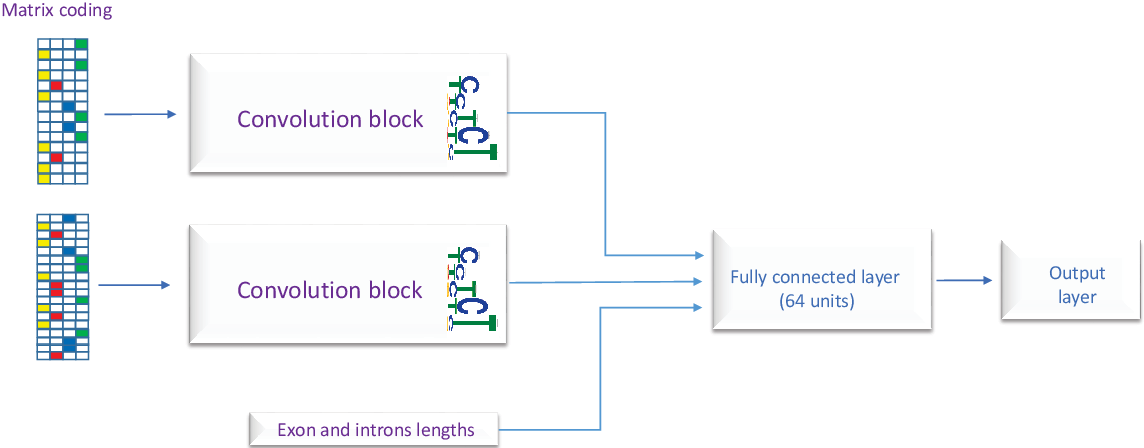
\includegraphics[width=0.7\textwidth]{../visualizations/ch4-methods/dsc_architecture.png} 
	\caption{
		Architecture of DSC \cite{dsc}. The one-hot encoded sequences are fed into two convolutional blocks which generate features that are concatenated with the exon and intron lengths and used by a fully-connected layer to obtain the classification output.
	}
	\label{fig:dsc_architecture}
\end{figure}

This model is the same as the Deep Splicing Code (DSC) model from \cite{dsc} and is based on CNNs.
CNNs are useful when the input data contains spatially invariant patterns. Since images are fundamentally made up of small, spatially invariant patterns which can be combined into more complex patterns, CNNs have been extremely successful in Computer Vision.\\
CNNs are also extremely promising for the application to nucleotide sequences: \\
1) We can expect to find motifs in the input sequence. Motifs are often represented as position weight matrixes (PWMs). The kernels used in CNNs can be interpreted as PWMs with learnable weights, i.e., the model can automatically learn to recognize important motifs.\\
2) These motifs may be found at different positions in the input sequence. Due to CNNs being spatially invariant they will be able to detect motifs at any position in the input sequence. \\
Keeping this motivation in mind, the first model extracts features from the two input sequences using CNN-based blocks. A CNN feature extraction block with the same architecture but independently learned weights is used for each input sequence. This is to accommodate the model learning to extract different features from the exon start and exon end sequence. The extracted features are used by a shallow MLP to obtain the final classification. 

Concretely, a CNN block consists of three convolutional layers. The first convolutional layer has a window size of 7 units and 32 filters, the second has a window size of 4 units and 8 filters and the third has a window size of 3 units and 8 filters. Each convolutional layer is followed by a dropout layer with dropout probability 0.2 to reduce overfitting [cite dropout], a ReLU activation layer and a max-pooling layer with stride and window size 2 to extract the most salient features. The hyperparameters for this model were chosen with grid search by \cite{dsc}. As we are dealing with inherently 1-dimensional textual data instead of inherently 2-dimensional image data, 1D convolution layers are used.



%https://stats.stackexchange.com/questions/288261/why-is-max-pooling-necessary-in-convolutional-neural-networks
%no one knows why max-pooling works

The extracted features for both genomic sequences are concatenated along with the normalized exon and flanking introns and input to a fully connected layer with 64 neurons. A ReLU activation function, as well as a dropout layer with probability 0.5, is applied to the output of this layer. The final layer takes in the 64 outputs from the previous layer, predicts a single value and is followed by a sigmoid activation layer.
a word on 1d convolution?
\subsubsection{Applying NLP techniques to genomic data}
Like text, genomic data is fundamentally a sequence of characters.
This makes it possible to apply techniques known from Natural Language Processing (NLP) to genomic data. This is an especially promising area of cross-pollination because of the large strides NLP has been able to make in recent years using deep learning.
Some of the most important milestones in NLP have been efficient embeddings via word2vec, applying RNNs to text as in seq2seq and extremely powerful and deep Transformers.\\
In this work, we will test the application of doc2vec (a derivative of word2vec) and seq2seq models to the task of alternative splicing classification. The current state-of-the-art transformer models, albeit very potent, usually require huge datasets in the order of millions of samples which aren't available for this task. While scaling them down might be an interesting avenue of research even heavily scaled-down models might still be over parametrized for the task as it has frequently been shown that very shallow networks (with less than 5 layers) perform best on genomic data. Additionally, our input sequences are very long; generally 140 tokens long. Initial tests showed that this also leads to memory problems when training on only one GPU, as the memory requirements of Transformers grows quadratically with respect to the length of the input sequence, further complicating their application. Due to these considerations, we chose to forego the evaluation of Transformer-based models in this study.
\subsection{D2V: MLP-based} \label{subsec:d2v}
%If I want to expand this section:
%Asgari, E., & Mofrad, M. R. (2015). Continuous distributed representation of biological sequences for deep proteomics and genomics. PloS one, 10(11), e0141287.
%Contains very good explanations / phrasings
\subsubsection{Introduction to word embeddings}
Word2Vec is a neural network-based model from Natural Language Processing (NLP) which provides a continuously distributed (vector) representation for each word within a sentence \cite{w2v1}\cite{w2v2}. The main idea of Word2Vec is that the meaning of a word is characterized by its context and therefore semantically related words will be similarly represented. The classic example is that

%Distributed representation has proved one of the most successful approaches in machine learning [6–10]. The main idea in this approach is encoding and storing information about an item within a system through establishing its interactions with other members. [biobvec]

$\vec{King} - \vec{Man} + \vec{Woman} ~= \vec{Queen}$
when adding the Word2Vec representations of the respective words.
Doc2Vec is an extension of Word2Vec which can handle variable length texts (such as paragraphs and complete documents) \cite{d2v1} \cite{d2v2}. It returns a fixed-length representation independent of input size.

\subsubsection{Training}
To train word2vec or doc2vec a large corpus of unlabelled data is needed. As we are training on genomic data, the largest corpus is the complete genome itself. The complete human reference genome GRCh38 \cite{hg38} was obtained from UCSC \cite{ucsc}.\\ %http://hgdownload.soe.ucsc.edu/goldenPath/hg38/chromosomes/
During training on text data, the corpus is split into documents which are ideally semantically meaningful (like paragraphs). Due to memory limitations and due to corresponding to the average gene size \cite{bionumbers}, we split the genome into sequences of 28,000 nucleotide sequences. However, tests with sequences of length 10,000 showed that this boundary length does not seem to affect model performance in a meaningful way.
\subsubsection{Using k-mers}\label{subsubsec:kmers}
Naively applying word2vec or doc2vec to genomic data would mean treating each nucleotide as a token. Drawing the parallel to natural language, this would mean wanting to embed each character in a word. However, a single character or nucleotide (which on top comes from an alphabet of only four characters) does likely not contain enough information by itself. Therefore, it is desirable to embed a k-mer.
One major difference between text and genomic data is the single-token complexity: a word contains far more information than a single nucleotide.
Multiple studies have explored this issue and found 3-mers to perform the best. %TODO:[add quotes from IEEE, IEEE itself]
 We follow their recommendation in this work and split each sequence of nucleotides into overlapping 3-mers. Overlapping means that in the case of the sequence 'AACGAT' the resulting overlapping 3-mer sequence is 'AAC', 'ACG', 'CGA' and 'GAT'. Therefore, the 28,000 nucleotides long pre-training sequences are split into overlapping 3-mer sequences (sentences) of length 27,998.
\subsubsection{Pre-training of word embeddings}
The pre-training for word2vec uses a shallow neural network with an input, hidden and output layer. If the continuous bag-of-words technique (CBOW) is used, all words in a window except the current word are given as input and the target output is the current word. Typical window size is 5. % TODO[WHAT DOES THE HIDDEN LAYER LOOK LIKE? -- could honestly skip this]
If the skip-gram technique is used, only the current word is given as input and the task is to predict the surrounding words in the window. Doc2Vec works similarly. In the CBOW equivalent called distributed memory (DM), a document identifier (usually just an integer enumerating all documents) is given as additional input. In the skip-gram equivalent distributed bag of words (DBOW), the current word is replaced by the document identifier and the task is to predict all words in the window. All four different training methods are visualized in Figure \ref{fig:w2vd2vtrainingvariants}.\\
There is no clear choice for when which training method should be used for Word2Vec or Doc2Vec as they tend to perform similarly. However, DM (and also CBOW) preserve the order of words and as the order of words (3-mers) is likely significant, we chose DM as pre-training method.
Pre-processing the human genome like above and using the DM training method, we trained the Doc2Vec model to output a 100-dimensional embedding for each document.
\begin{figure}
	\centering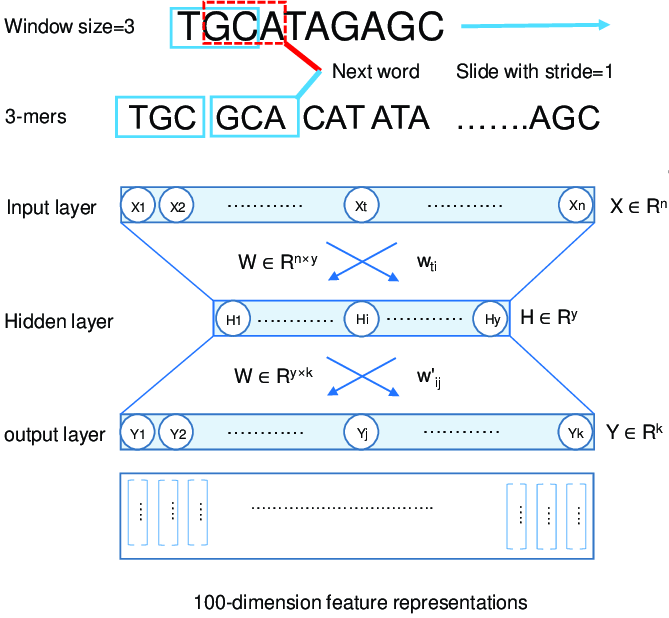
\includegraphics[width=1\textwidth]{../visualizations/ch4-methods/d2v_training_cropped.png} 
	\caption{
		Process by which the 100-dimensional embeddings are obtained \cite{d2vsplicing}: the input sequence is split into overlapping 3-mers which are then fed as input into the pre-trained d2v model. 
		% TODO add sentence how 100-dimensional embedding is actually obtained
	}
	\label{fig:d2vtraining}
\end{figure}


\begin{figure}
	\centering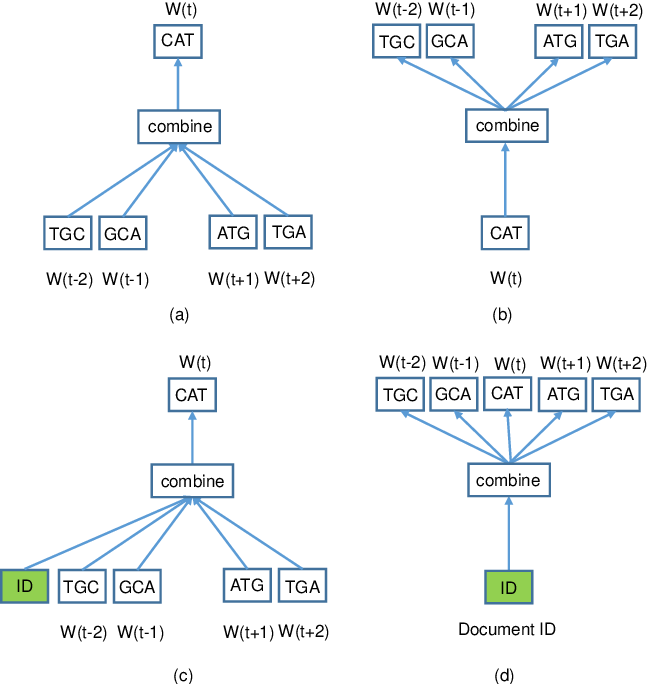
\includegraphics[width=1\textwidth]{../visualizations/ch4-methods/w2v_d2v_training_variants.png} 
	\caption{
		The four possible training algorithms for w2v and d2v models \cite{d2vsplicing}: (a) CBOW, and (b) skip-gram for w2v, and (c) DM and (d) DBOW for d2v. 
	}
	\label{fig:w2vd2vtrainingvariants}
\end{figure}

\subsubsection{Analyzing the obtained embeddings}

\begin{figure}
	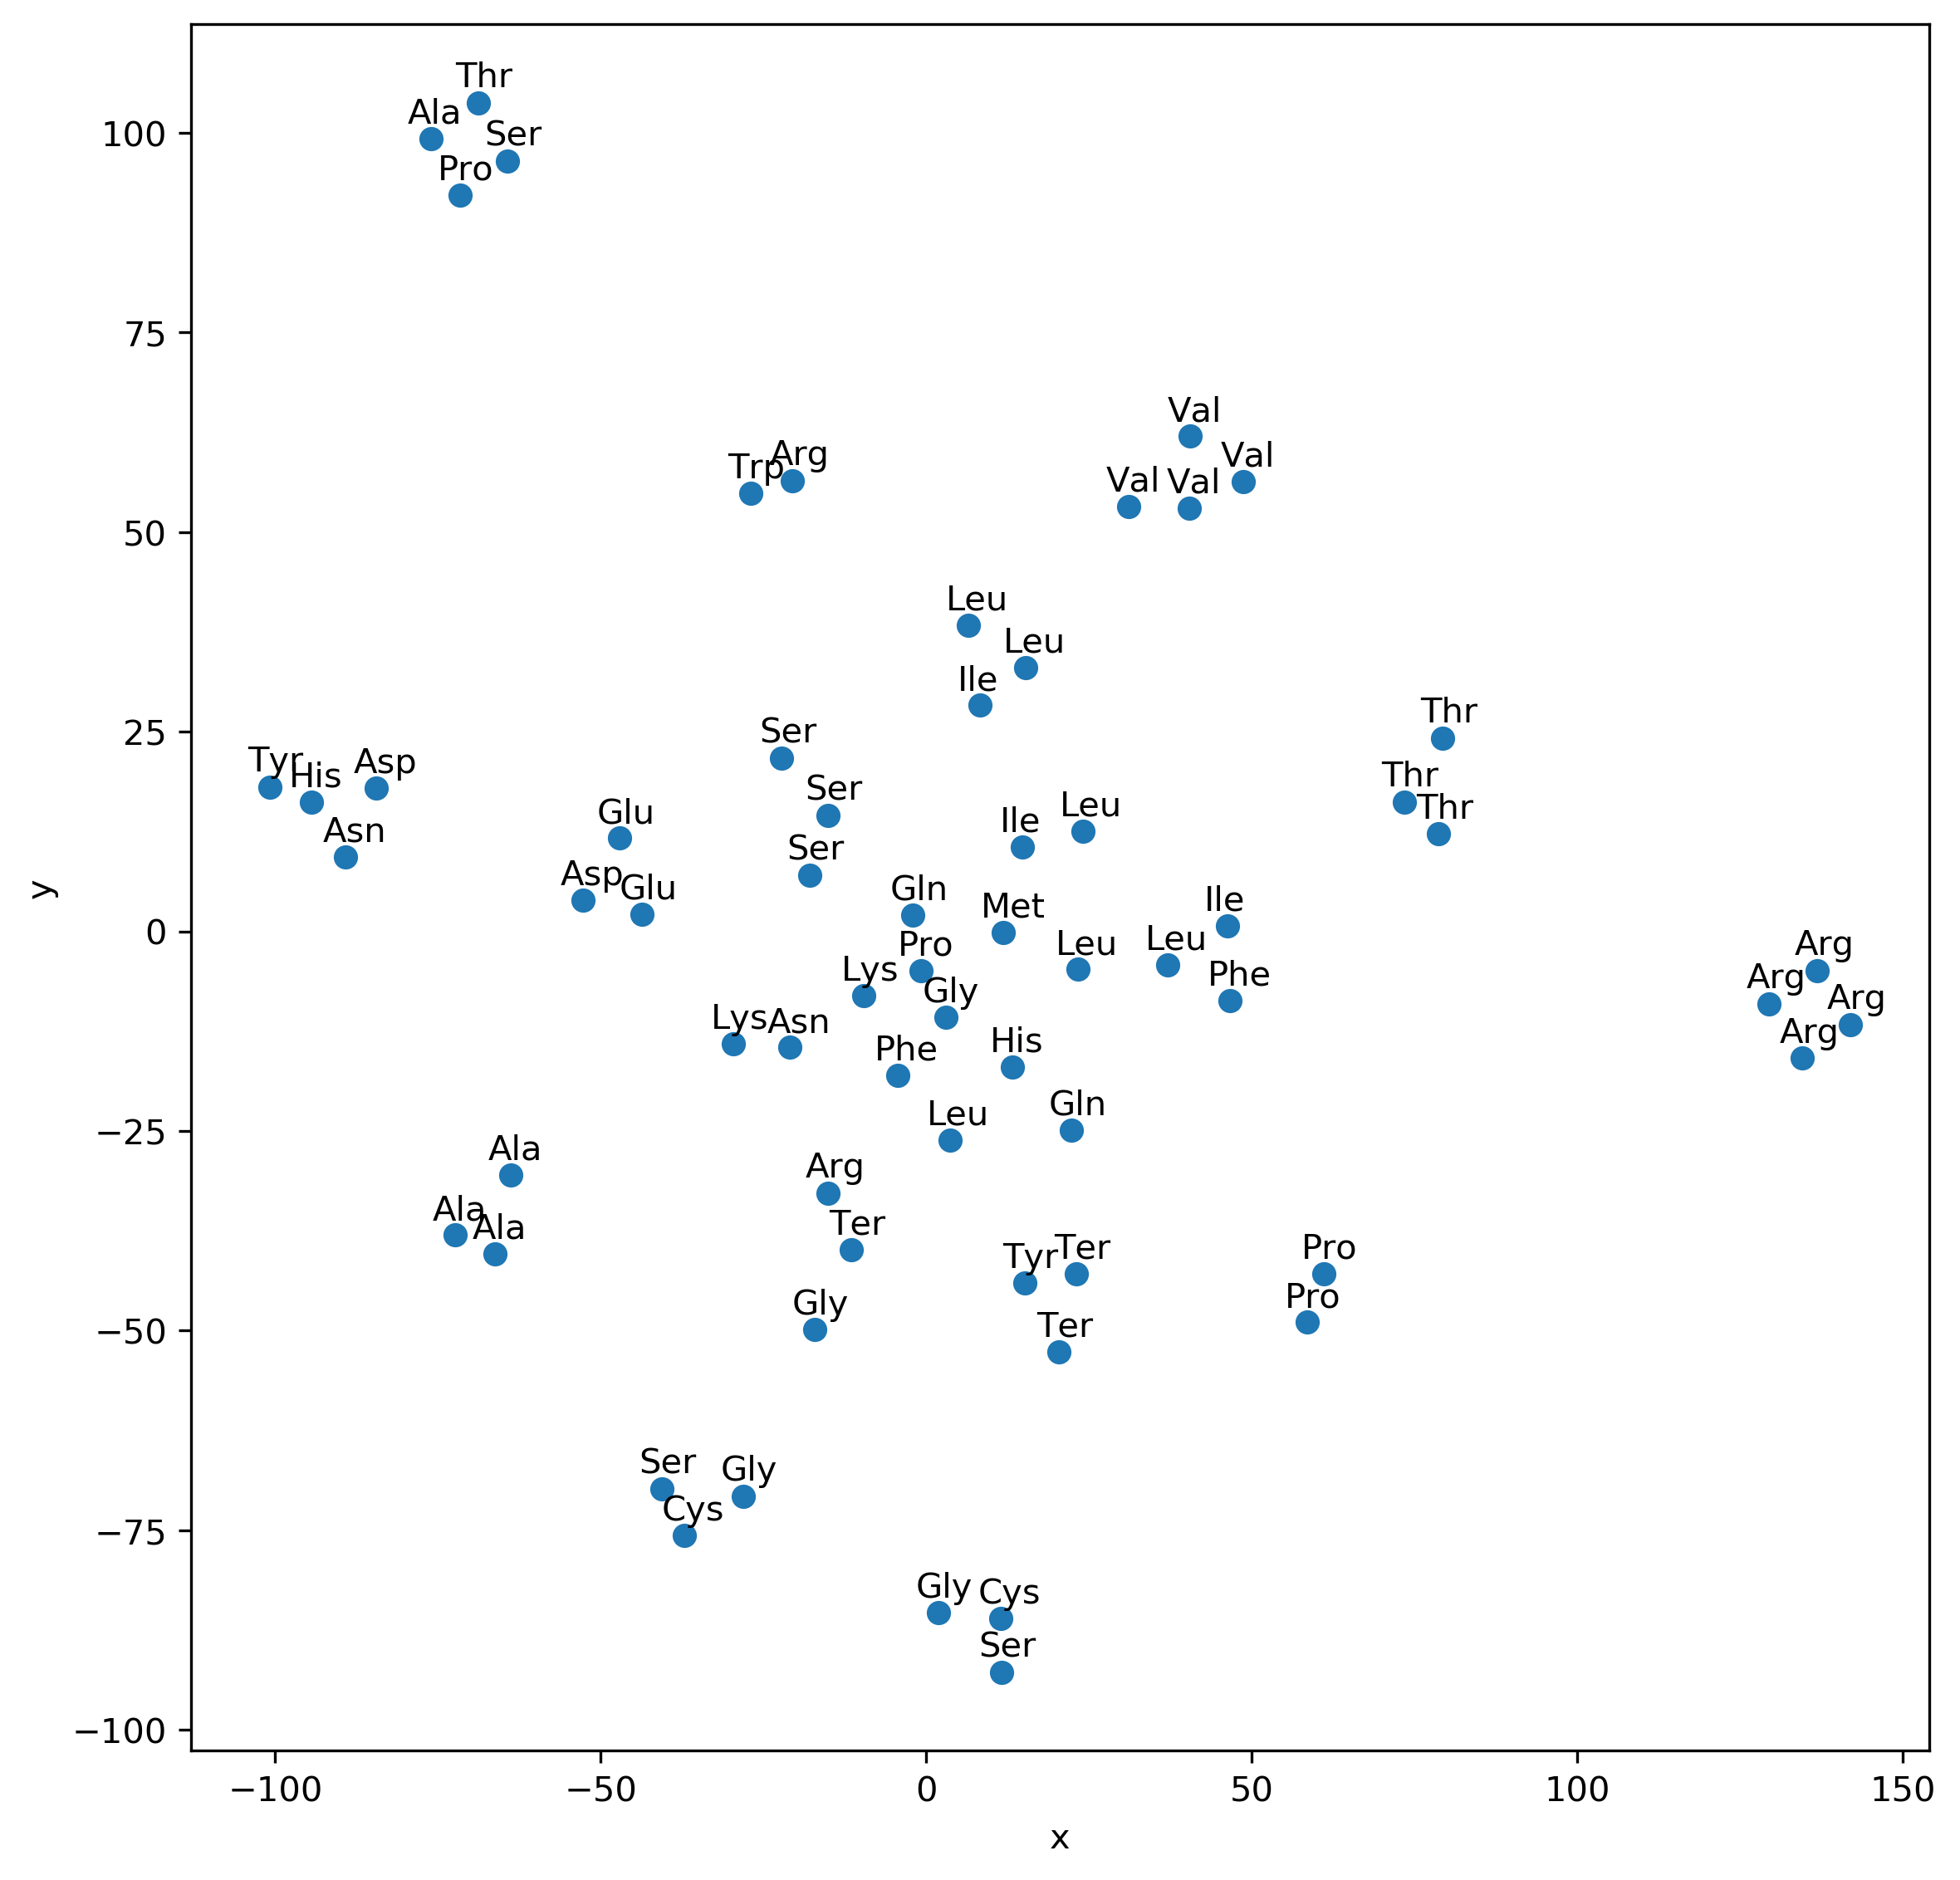
\includegraphics[width=0.5\textwidth]{../visualizations/ch4-methods/tSNE-d2v.png} 	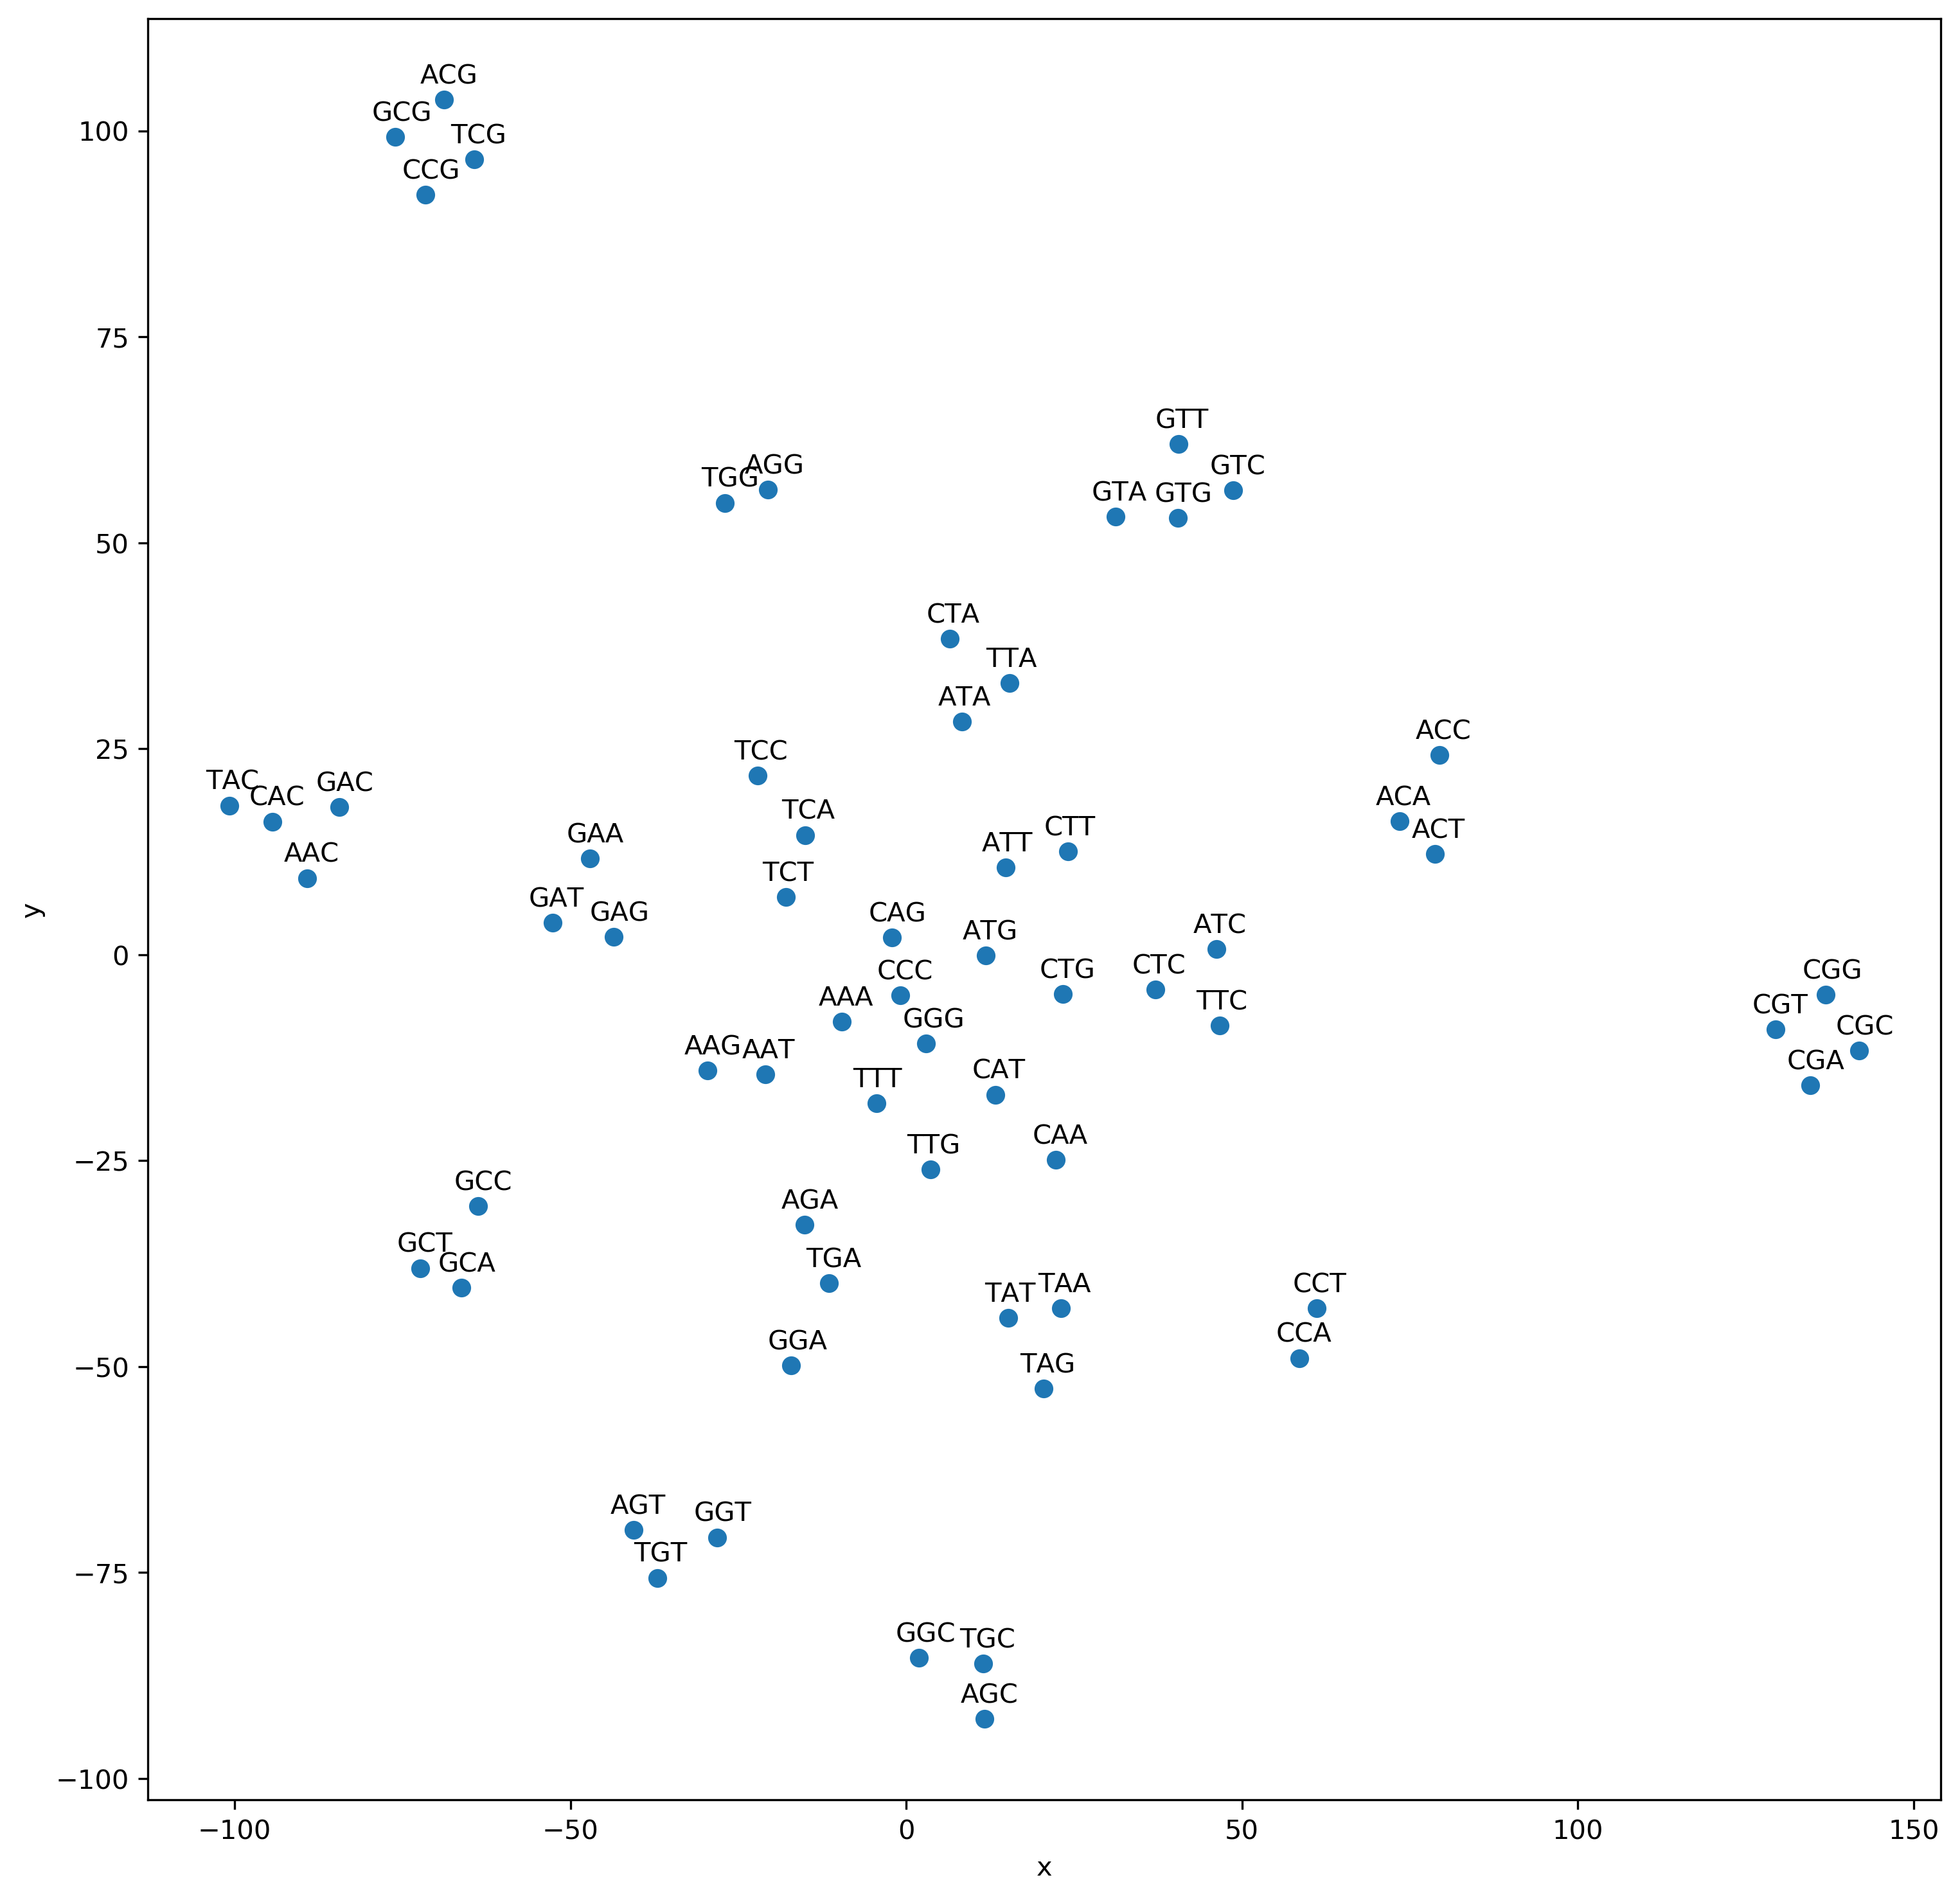
\includegraphics[width=0.5\textwidth]{../visualizations/ch4-methods/tSNE-d2v_bases.png} 
	\caption{
		The 2-dimensional embeddings obtained by applying t-SNE to the 100-dimensional learned representations of all 64 possible 3-mers. Left shows the codons encoded by the 3-mers, right shows the actual 3-mers.
		 }
	\label{fig:tsne}
\end{figure}

We visualize the embeddings for all 64 possible 3-mers using Stochastic Neighbor Embedding (t-SNE) \cite{tsne} in Figure \ref{fig:tsne}.

Doc2Vec is trained to map words (3-mers) which occur in a similar context to similar representations. We observe that this often translates to mapping the same amino acids to similar representations. There are some instances when different amino acids are mapped together like the quartet Ala, Thr, Pro and Ser in the top-left corner. Displaying the 3-mers associated with the amino acids, that this likely occurs because these different amino acids share two out of three nucleotides at the same positions. We take this visualization as an indication that Doc2Vec was able to learn biologically useful embeddings for the overlapping 3-mers.
[maybe] Making use of these pre-trained embeddings, each 140 nucleotide input sequence is split into overlapping 3-mers and mapped to a 100-dimensional vector. Like in the other models, a shallow MLP using these sequence features in conjunction with length features for classification.
\subsubsection{Inference} \label{subsubsec:d2vinference}
During inference, the Doc2Vec model outputs 100-dimensional embeddings for each input sequence. These, along with the length features, are fed into the shallow MLP for classification. The shallow MLP consists of two layers with 16 and 8 neurons each respectively followed by a dropout layer with dropout probability of 0.2.


%[discussion of the tsne embeddings here]
%research on what to write:
%doc2vec will map words (3-mers) which are used in similar contexts to similar representations
%wil: codon usage bias; not all encodings of a codon will be used with the same frequency
%the bias of codon usage at exon boundaries
%Laurence Hurst paper looks at biases in the first and last 30 nucleotides within an exon



\subsection{BiLSTM + Attn} \label{subsec:bilstm}
% TODO: I AM DRASC
\subsubsection{Seq2Seq} \label{subsubsec:seq2seq}
Sequence-to-sequence learning (Seq2seq) \cite{seq2seq} is a general deep learning-based framework for mapping one sequence to another. The first part of the framework is an encoder which processes the input symbol-by-symbol and produces a vector representation for each input symbol. The second part is a decoder which predicts the output sequence symbol-by-symbol based on the representation(s) computed by the decoder. In the first timestep, the decoder uses the last output of the encoder and in all other timesteps, it uses its own output from the previous time step as input. The encoder and decoder are typically RNN-based networks such as LSTMs \cite{lstm} or GRUs \cite{gru}. Encoder and decoder are jointly trained to maximize the probability of correct output. This framework has been particularly successful in machine translation (MT): for instance, Google announced in 2016 that it started using them for their MT \cite{googlemt2016}. Figure \ref{fig:encdec} visualizes the working of an encoder-decoder model.

\begin{figure}
	\centering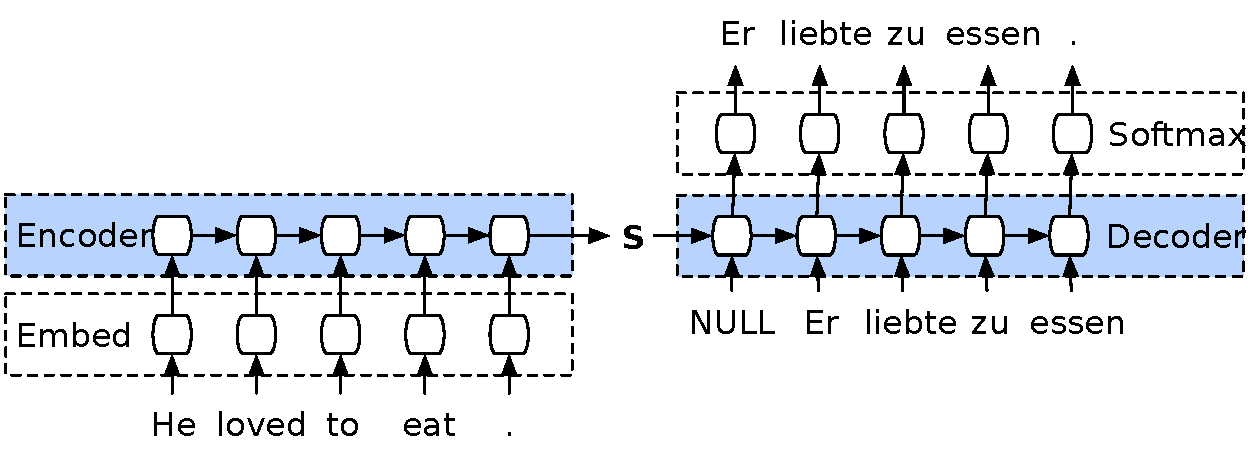
\includegraphics[width=0.9\textwidth]{../visualizations/ch4-methods/enc_dec.pdf} 
	\caption[bla.]{An encoder-decoder model \cite{ruderencdecgraphic} translates the English sentence 'He loved to eat' to the German sentence 'Er liebte zu essen'. The decoder takes the last hidden cell state of the encoder as initial input and generates the output token-by-token. The decoder takes its own previous output as prompt for the next output and stops generating output token when it generates a '.'-token. }
	\label{fig:encdec}
\end{figure}

%Sutskever, I., Vinyals, O., & Le, Q. V. (2014). Sequence to sequence learning with neural networks. In Advances in Neural Information Processing Systems.
%https://smerity.com/articles/2016/google_nmt_arch.html
%https://ruder.io/a-review-of-the-recent-history-of-nlp/index.html#2013wordembeddings
\subsubsection{Are you paying attention?}
In the original Seq2seq framework, only the last state of the encoder is passed to the decoder. This means that the encoder needs to encode all of the information observed in the input sequence into its last state. While theoretically possible, \cite{attention} hypothesized that this informational bottleneck hampered performance in practice. They proposed removing this bottleneck via introducing attention. Attention is a mechanism whereby the decoder can look at all the representation generated by the encoder at once and can 'choose' to focus on the most important ones. Introducing attention lead to large performance gains across Seq2seq-based models and quickly became standard practice. The attention mechanism also adds interpretability to the model because it indicates which parts of the input sequence are most crucial for the model's prediction. Figure %[TODO]
 visualizes what parts of an input sequence a model is paying attention during an MT task. Attention is one of the most important innovations in deep learning research in recent years. For instance, the current state-of-the-art Transformer models \cite{allyouneed} \cite{bert} \cite{gpt3} forego recurrent networks completely and solely use attention within the encoder and decoder components.
However, as justified earlier, we won't focus on these models due to issues of scaling and the sufficiency of shallow networks for genomic prediction tasks.
%Bahdanau, D., Cho, K., & Bengio, Y. (2015). Neural Machine Translation by Jointly Learning to Align and Translate. In ICLR 2015.
%could also use graphics from this
%another attention reference: https://arxiv.org/pdf/1508.04025.pdf
%https://3.bp.blogspot.com/-3Pbj_dvt0Vo/V-qe-Nl6P5I/AAAAAAAABQc/z0_6WtVWtvARtMk0i9_AtLeyyGyV6AI4wCLcB/s1600/nmt-model-fast.gif
%alternative: https://machinetalk.org/2019/03/29/neural-machine-translation-with-attention-mechanism/
Attention is a very general mechanism not limited to the Seq2seq framework and different forms of it (such as additive \cite{attention} or multiplicative attention \cite{allyouneed}) are used in practice. It can theoretically be useful for any task where a model needs to make a decision based on certain parts of an input.
%[transformer here and why I don't use it]
%[More applications of attention]
%It has been applied to constituency parsing (Vinyals et al., 2015)
%, reading comprehension (Hermann et al., 2015)
%, and one-shot learning (Vinyals et al., 2016)
%, among many others. The input does not even need to be a sequence but can consist of other representations as in the case of image captioning (Xu et al., 2015)
%, which can be seen in Figure 12 below
\subsubsection{Integrating attention}
Taking inspiration from the successful application and improved interpretability of the Seq2seq framework with attention in other domains, we also adopt it for constitutive exon classification. We now describe the modifications we made to initial Seq2Seq and attention set-up known from MT for our our context. In particular, we describe the attention mechanism in more detail as necessary for our second modification.
\subsubsection{Modification 1: MLP instead of a recurrent decoder}
As the name implies, models based on the Seq2seq framework take a sequence as input and give a sequence as output. This is achieved via using a recurrent decoder which outputs symbols until it outputs an <EOS> (end-of-sentence, e.g. a '.') token (in the case for MT, similar for other domains). However, in our case, the output will always be a single scalar: the classification of the exon as constitutive or alternatively spliced. Thus, we don't require a recurrent decoder and instead use a shallow MLP for classification of the encoder features.
\subsubsection{Modification 2: Attention with a learned query vector}
%todo fix this section (with graphics etc) when you have results of new attentio nexperiments
The most common form of attention (multiplicative or dot-product attention), makes uses of conceptual queries and key-value pairs. A given query is compared to all keys by computing a similarity score between the query and each key via the dot-product. The similarity scores are normalized through the use of a softmax layer. The normalized similarity scores are also commonly called the attention weights; keys similar to the query are weighted more. The output of the attention layer for a given query and input sequence is then the weighted vector sum obtained by multiplying each value by the attention weight of its respective key.
Putting the above intuition into formulas, the (dot-product self-) attention mechanism can be described using the following equations:
$$Q, K, V = IW^Q, IW^K, IW^V$$
The query, key and value matrices Q, K and V are computed by multiplying the input with query, key and value parameter matrices $W^Q$, $W^K$ and $W^V$.
where $$W^Q,W^K, W^V \in \mathbb{R}^{in \times out}$$,
and $Q,K, V \in \mathbb{R}^{l \times out}$. $in$ corresponds to the number of features of each element in the input sequence to the attention layer, $out$ corresponds to the number of features in the output of the attention layer. $l$ corresponds to the number of elements in the input sequence to the attention layer.
Attention can be then computed as:
$$Z = attention(I) = softmax(QK^T)V$$
where $Z \in \mathbb{R}^{l \times out}$. The input $I$ is a concatenation (along the first dimension) of the representations given by the two BiLSTMs.
Note that this makes use of the fact that $Q\cdotp K = QK^T$ where $$\cdotp$$ denotes the dot product.\\
%This form of attention is also visualized in Figure !](https://jalammar.github.io/images/t/self-attention-matrix-calculation.png) and ![
%from https://jalammar.github.io/illustrated-transformer/
%todo: remove this division by square-root -- maybe ask Kuba how to photoshop this away
As shown, multiplicative self-attention computes a separate query for each input token. It is called self-attention because it allows a sequence to pay attention to 'itself'. (Unmasked) self-attention is mainly used in the encoder part of Transformer architectures to improve the representation for each word.\\
However, our objective in using attention is not to improve the representation for each symbol in a sequence (this is the task of the BiLSTM), but to select the most important features from an input sequence. The conceptual query for our task is also always the same independent of input: is this exon constitutively spliced or not?
%thought: this also naturally happens in seq2seq models when they use attention -- how is what I am doing differently?
Thus, we adapt the attention mechanism so that we learn a single, input-independent query ${Q}^* \in \mathcal{R}^{1 \times out}$. The output of the attention layer is now computed as:
$$Z^* = {attention}^*(I) = softmax({Q}^*K^T)V$$

%decided against explaining innovation as two-points with (1) one query and (2) independent of input because I felt unsure of (2)

where $Z^* \in \mathbb{R}^{1 \times out}$. Note that the query matrix ${Q}^*$ is directly learned in the attention block and not multiplied with the input, giving rise to its input independence. The output $Z$ is now a weighted sum of the nucleotide representation in the input sequences which the model deemed most crucial to pay attention to.
\subsubsection{Putting it all together:} 
Like a Seq2Seq model, an RNN-based Encoder is used to capture a representation of the input sequence. We select the most important representations of the input using the modified attention mechanism we introduced. Instead of a recursive decoder, we use a shallow MLP for classification based on the selected features.
One detail not mentioned yet is that the input to the BiLSTM blocks is a dense 4-dimensional embedding of the one-hot encoded sequences. This embedding is the same for each sequence and jointly learned during training. This extra embedding layer is included as previous works \cite{embeddingneeded} have shown that otherwise, the model might suffer from limited generalization performance caused by the sparsity of the one-hot encoded representation. 

\begin{figure}
	\centering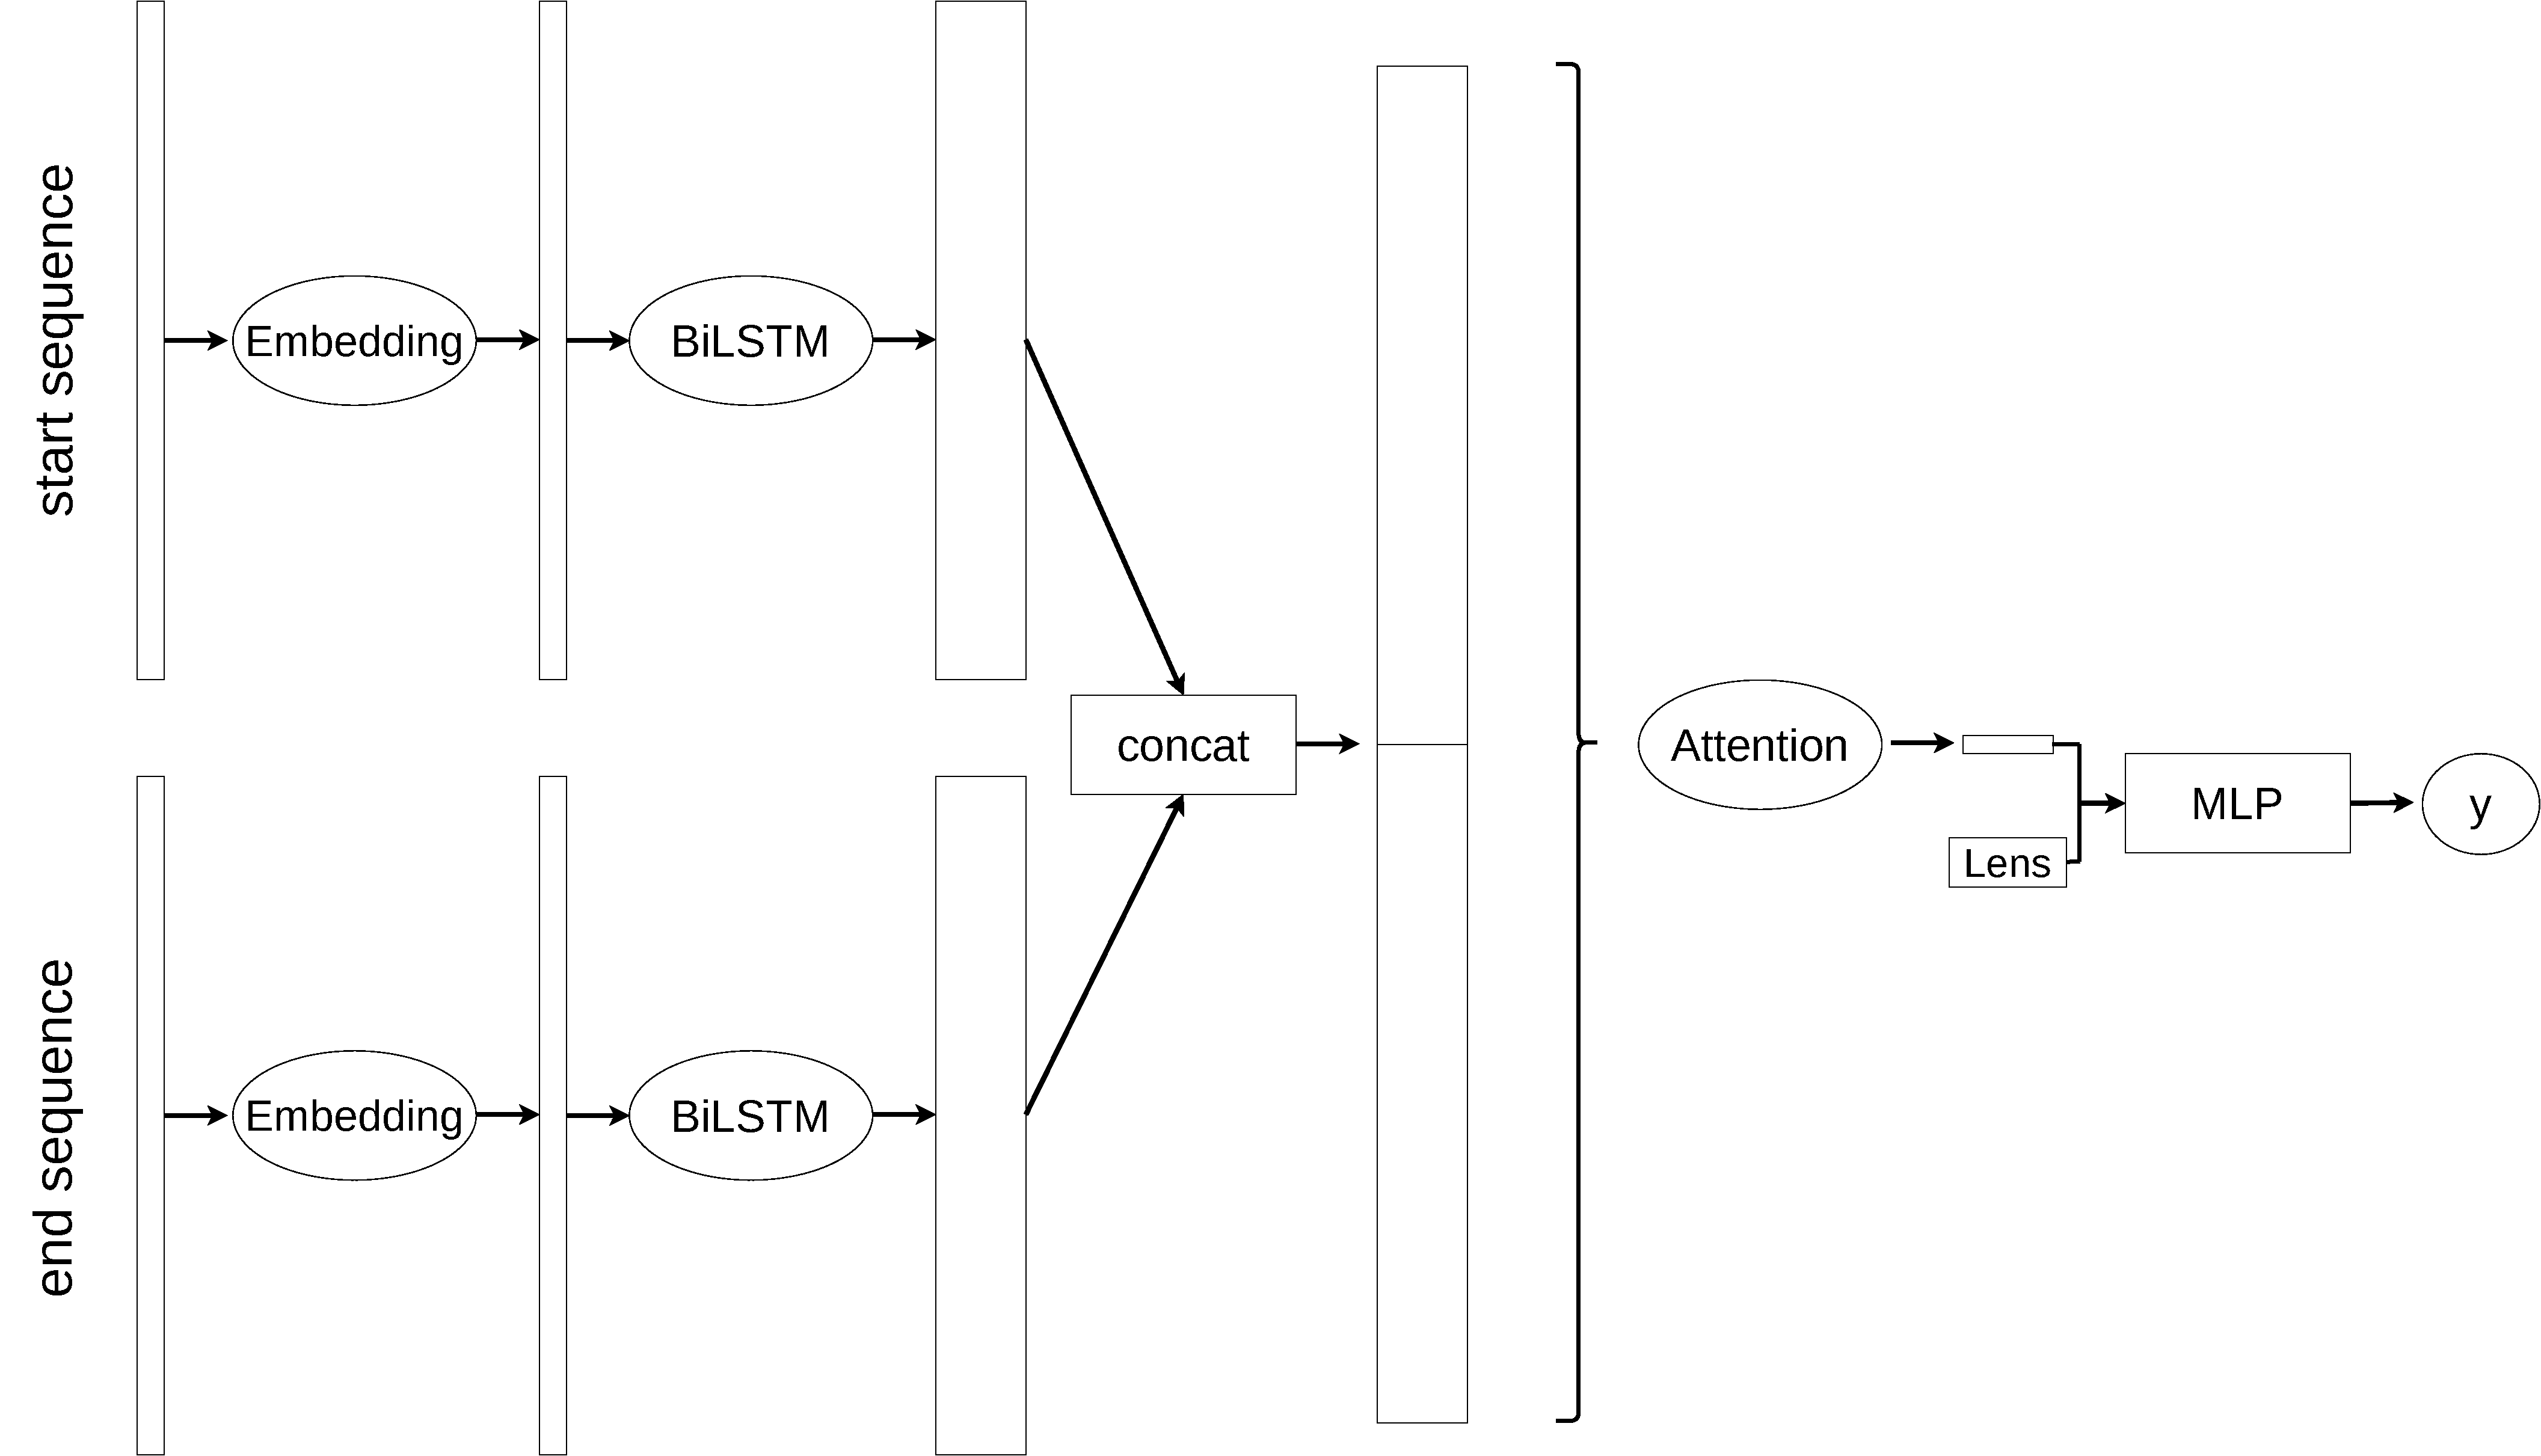
\includegraphics[width=1\textwidth]{figures/AttnBiLSTM.pdf} 
	\caption{Architecture of the new attention-based model we introduce. }
	\label{fig:attnbilstm}
\end{figure}

\subsection{Alternative implementations of attention} \label{subsec:alternative_attention}
In the following, we introduce multiple extensions which were attempted which didn't lead to improved results. For most of these, initial results clearly showed that the results weren't improved by using them. As such, we didn't test these extensions more extensively than initial experiments because we felt the initial results were already instructive enough and no further investigation was warranted. Thus, the analysis of the results won't be as extensive as for the extensions which worked.
\subsubsection{No query} \label{subsubsec:noquery}
As the query matrix ${Q}^*$ is already the same independent of the exact input sequence, it could be possible to drop it and compute the attention weights sorely based on the key matrix K.
This is possible by learning a key weight matrix $W^{K^*} \in \mathcal{R}^{in \times 1}$ and computing attention as:
$$K^* = IW^{K^*}$$
$$Z^{} = {attention}^{}(I) = softmax(K^*)V$$
where $K^* \in \mathbb{R}^{l \times 1}$ and $Z^{**} \in \mathbb{R}^{1 \times out}$
However, in initial experiments, the attention** mechanism performed significantly worse than the attention* mechanism. The extra representational capacity by having a query matrix seems to be important for performance.
\subsubsection{Multiple attention heads} \label{subsubsec:heads}
Having one set of query, key and value matrices limits the model to one representational subspace (one way of 'interpreting' the input). It might be useful for the model to have multiple representational subspaces. This is usually achieved via $h$ different sets of query, key and weight matrices $W^Q_1, W^Q_1, W^Q_1, \dots W^Q_{h}, W^Q_{h},W^Q_{h}$ producing multiple outputs $Z_0, \dots, Z_{n\_h}$.
The final output matrix $Z_{final} \in \mathcal{R}^{l \times out}$ is then computed as:
$$Z_{final} = concat(Z_1, \dots, Z_{h}) W^O$$
where the concatenation occurs along the second dimension and $W^O \in \mathcal{R}^{out * h \times out_{new}}$. $out_{new}$ represents the new output dimension of the attention layer, which is arrived at by combining the dimensions of the multiple attention heads.

%thought: might change this up a little, would require a bit more implementation effort than previously thought (eg. initial attention dimension should be divided by 3) or requires the assumption that out == $out_new$ (I think I will choose this one, but not certain)
\subsubsection{Convolution in attention heads} \label{subsubsec:attention_conv}
As was previously discussed in the motivation for splitting the input sequence into overlapping 3-mers in \ref{subsubsec:kmers}, the information contained in a single nucleotide is very low. This motivated \cite{ghentransformers} to apply an additional 1D convolution to the query, key and value matrices Q, K and V. This extension can be understood as an alternative to splitting the input into k-mers and provided better results than splitting the input into k-mers when using a Transformer network for a genome annotation task in \cite{ghentransformers}.
Keeping in mind the modification of directly learning the query matrix, this leads to:
$$K_{conv}, V_{conv} = conv(K), conv(V)$$
$$Z^* = {attention}_{conv}^*(I) = softmax({Q}^*K_{conv}^T)V_{conv}$$
where the K and V are both fed through the same convolutional layer.
The number of convolution filters and padding are chosen so that the dimensions of the K and V matrices don't change, that is, $K_{conv}, V_{conv} \in \mathbb{R}^{l \times out}$.
One more detail regarding the application of this extension: to incorporate the domain knowledge that the input sequences to the neural network come from different places in the genome, we made sure that the convolution did not mix the information between the two sequences. To achieve this, the following computation actually took place :
$$K^{start}, K^{end} = I^{start}W^K, I^{end}W^K,$$
$$K^{start}_{conv}, K^{end}_{conv} = conv(K^{start}), conv(K^{end})$$
$$K_{conv} = concat(K^{start}_{conv}, K^{end}_{conv})$$
where the 'start' and 'end' superscript respectively refer to the sequence around the start and end of the exon. The concatenation is along the first dimension (so the length of the sequences). The analogue computation was done for $V_{conv}$.\\
TODO: add this separately to results section
Testing this extension on the HipSci MAJIQ dataset didn't lead to improved results. Although the convergence speed increased rapidly (from around 180 epochs to 20 epochs), we also observed heavy overfitting. To alleviate this, we added dropout and batch normalization layers. After adding two dropout layers with a high dropout probability (one after computing the attention weights and one after the convolution layers with p=0.5 each) and setting the convolutional filter size to no higher than 3, overfitting issues ameliorated. However, after adding these layers convergence was no faster than for the case without convolutional layers and the performance did not improve. Thus, for the sake of a simpler model, we opted to not use this extension for the rest of the experiments.
Reasons for why this extension did not work might be related to the use of a recurrent encoder as well as task differences compared to \cite{ghentransformers}:
\begin{enumerate}
	\item Although we process the input at single-nucleotide resolution, the use of a BiLSTM means that the encoder is aware of the nucleotides which precede and follow it. Therefore, information about the neighbouring nucleotides is likely already represented in the representation for a given nucleotide. This is in contrast to a Transformer model where the layers are non-recurrent and only work at single-symbol resolution. Thus, the convolutional layers likely don't give the model a lot more flexibility.
	\item In \cite{ghentransformers}, the task is a full genome transcription start site annotation. Therefore, in a sense, their task occurs at the inter-gene level while our task occurs at the intra-gene level. This likely means that the motives the model has to consider generally span more nucleotides and giving the model more capacity to integrate over multiple nucleotides is more crucial. In contrast, the single-nucleotide resolution of our model may be necessary to help it identify the more fine-grained motifs which influence splicing. Thus, these differences likely also influenced the performance differences when using the convolutional attention layer extension in the different models.
%		they: 3000 nucleotides, convolution filter of 7
\end{enumerate}


A small implementational detail regarding the attention blocks: the query, key and value parameter matrices are implemented via a linear layer with the appropriate dimensions. These also learn bias weights which are added to the output by default. While in theory the bias weights should be turned off to implement exactly the shown formulas, in practice other attention mechanism implementations leave these turned on \cite{annotatedtransformer} and so we follow suit. Thus, to be precise, the query, key and value computation should be:
%TODO this formula of the attention mechanism
%   old motivation:
%The architecture of this model can be motivated in two ways:
%1) Similar to DSC, we use two blocks for feature extraction. However, incorporating the knowledge that our input data is a sequence, we use an RNN for this feature extraction. In particular, under the assumption that bidirectional context is important for this task, we use bidirectional LSTM (BiLSTM). Like DSC, a shallow MLP uses the obtained features of both blocks for classification.
%2)
%The final model is very similar to the current state-of-the-art splicing code for predicting the inclusion rate of a cassette exon [distributed], as introduced in [related works].
%maybe: (could make my motivation seem shallow)
%This is a standard LSTM architecture and a similar architecture have been successfully applied to the related task of finding new splice junctions. [https://arxiv.org/pdf/1512.05135.pdf, https://www.sciencedirect.com/science/article/pii/S0010482519304135]
%simple feature extraction + classification model as eg in [https://www.researchgate.net/figure/An-example-of-bidirectional-LSTM-tagger-architecture_fig1_330276457 ] -- 5 citations

For this model, the hyperparameter space was a lot larger and model performance was very sensitive to the hyperparameter choice. The most crucial hyperparameters were the number of encoder dimensions and the number of dimensions of the attention layer. Hyperparameters were optimized via grid search on the HipSci MAJIQ dataset.

putting model parameters into the text instead of a table:
Concretely, each LSTM block consists of a BiLSTM with one (?) layer which outputs 50 features.
The shallow MLP used for classification uses a single layer with 128 (?) neurons and is followed by a dropout layer with dropout probability of 0.5.


\section{Training and implementation details} \label{sec:implementation_details}
\subsection{Implementation} \label{subsec:implementation_details}
All models, except the Doc2Vec network, were implemented using the PyTorch library (version 1.5.0) \cite{pytorch}. It was chosen (over TensorFlow) as the main author already had more experience with PyTorch. The Doc2Vec model was implemented using the gensim library (version 3.8.3) \cite{gensim}. The data processing was done using a mixture of Python and Bash scripts as well as the software tools MAJIQ and SUPPA described in section \ref{subsubsec:majiq} and \ref{subsubsec:suppa}. The complexity induced by the use of a large number of different datasets and data processing methods was handled by standardizing the shape of the final training samples. Even though 12 different datasets and 3 different models are used, the codebase contains only 2 different data loader and trainer classes.


The structure of the repository was based on the PyTorch Deep Learning Project template available at \url{github.com/victoresque/pytorch-template}. This template provides access to abstract classes for data loaders, trainers and the models themselves. These abstract classes already contain a lot of the implementation-independent code to log results and train and save models. These abstract classes can then be extended with implementation-specific code as e.g. exact data formats. Using this structure avoids the duplication of a lot of boilerplate code.\\
To run an experiment, the experimental settings are defined in separate JSON files. This allows for easy and unambiguous reproduction of results. All experiments for whom results in this study are shown are available as JSON files that define the exact parameters used.
The code repository itself contains multiple README which go into more details towards the structuring and using of the code and also define naming conventions.\\

TODO: total code base contained roughly ... lines of code. the majority of these were in preprocessing section [maybe exclude this]

\subsection{Training} \label{subsec:training_details}
The training was done using one NVIDIA GeForce GTX 1080 Ti GPU. This proved to be sufficient as initial exploratory experiments showed no advantage of using deep networks and the resulting networks used are all relatively shallow. The pre-training of the Doc2Vec model on the human genome took 3 hours. We randomly split each dataset into 10 folds; in a given run, 8 folds were used for training, 1 fold for validation and 1 fold for testing. Each model was trained with different folds 9 times.
The training time for training a single model once varied between 1 minute and 75 minutes (see [table with training times]). The models were trained with early stopping on the validation fold until they stopped improving for 15 epochs. This typically occurred after 70 - 150 training epochs.
Where we established in a base experiment that the variance for a given model was low between runs (lower than ~1%), we only trained the model in follow-up experiments once for practical reasons.
\subsubsection{Loss}  \label{subsubsec:loss}
All models were trained to minimize the binary cross-entropy loss:
$$\mathbb{L} = - (y \log(\hat{y}) + (1 - y) \log (1 - \hat{y}))$$
where the ground truth $y \in \{0, 1\}$ and the prediction of the model $\hat{y} \in [0, 1]$. The binary cross-entropy is the standard loss for training deep learning-based (binary) classifiers.
\subsubsection{Metrics} \label{subsubsec:metrics}
As in previous work \cite{dsc}, we evaluate all models using the Area under ROC curve (AUC). The AUC provides an aggregate measure of performance across all possible decision thresholds.
However, some of our datasets were unbalanced. This may lead to a degenerating behaviour where a model only predicts the majority class. Additionally, only looking at the AUC does not give a good sense of the .... specificity.. recall?
This is not captured by the AUC. \\
Thus, we also evaluated the F1 of our models when working with an unbalanced dataset as in the case of the HipSci-based dataset processed with MAJIQ.
The output of our models is a single, continuous scalar $\hat{y} \in [0, 1]$. As the AUC itself is an aggregate measure across all decision thresholds, we don't need to set it to a certain value that translates the continuous prediction into a discrete positive or negative class prediction. To compute the F1 score, we do. Naively, this threshold may be set to 0.5; that is, all outputs above 0.5 will be interpreted as a prediction of the positive class and all other outputs as a prediction of the negative class. However, this threshold may not be optimal to maximize the F1 score, especially when working with unbalanced datasets. We choose the threshold which maximizes the F1 score on the test set.



\begin{table}[h!]
	\centering
	\begin{tabular}{| l | c |} 
		\hline
		\textbf{DSC}\\
		\hline
		Kernel filters & 32, 8, 8 \\
		Kernel size & 7, 5, 3 \\
		Dropout (after fully-connected layer) & 0.5\\
		Neurons fully-connected layer & 64 \\
		Dropout (after convolution) & 0.2, 0.2, 0.2\\
		\hline
		\textbf{D2V}\\
		\hline
		Embedding dimension & 100\\
		Neurons (fully-connected layers) & 32, 8\\
		Dropout (fully-connected layers) & 0.2, 0.2\\
		\hline
		\textbf{BiLSTM + Attention} \\
		\hline
		Dense embedding dimensions & 4\\
		BiLSTM dimension & 50\\
		BiLSTM layers & 1\\
		Attention heads & 4\\
		Attention head dimension & 50\\
		Dropout (attention head) & 0.4 \\
		Attention layer output dimension & 100\\
		Neurons fully-connected layer & 128\\
		Dropout (after fully-connected layer) & 0.5\\
		\hline
	\end{tabular}
	\caption{Hyperparameters of the main models
	}
	\label{table:hyperparameters}
\end{table}

TODO: [mention respective model sizes here]
bilstm + attn 66861, dsc 20.001, d2v 6801

Exact hyperparameters used for training the models are given in table \ref{table:hyperparameters}.
The DSC, D2V and BiLSTM + Attn models respectively contain 20,001, 6,801, and 66,861 trainable weights. In absolute terms, all of these model are still small compared to models known from Computer Vision and Natural Language Processing. The number of training weights is also reflected in the training times with the models respectively taking between 5 to 30 minutes, 1 to 5 minutes and 15 to 75 minutes to train once (depending on dataset). 

 
%TODO; for destruction of EST the following may be interesting: Quantitative comparison of EST libraries requires compensation for systematic biases in cDNA generation
